% !TEX root = main.tex
\chapter{Πειραματικός Σχεδιασμός και Αποτελέσματα}
\label{chap:experiments}

Το κεφάλαιο αυτό παρουσιάζει την εμπειρική σύγκριση των τριών δειγματοληπτών Langevin ---
του Unadjusted Langevin Algorithm (ULA), του Metropolis-Adjusted Langevin
Algorithm (MALA) και του underdamped kinetic langevin με BAOAB splitting --- σε τρεις
κατανομές-στόχους που καλύπτουν ένα ελεγχόμενο φάσμα συμπεριφοράς ουράς:
μια κανονική Γκαουσιανή (εκθετικά ελαφριές ουρές), μια κατανομή Student-$t$ με
$\nu=5$ βαθμούς ελευθερίας (πολυωνυμικές ουρές με πεπερασμένη διακύμανση) και μια
τυπική κατανομή Cauchy (πολυωνυμικές ουρές χωρίς πεπερασμένες ροπές).
Αρχικά περιγράφουμε τον πειραματικό σχεδιασμό (Ενότητα~\ref{sec:exp-design}).
Στη συνέχεια παρουσιάζουμε τη μελέτη πλέγματος παραμέτρων
(Ενότητα~\ref{sec:grid-study}), εξετάζουμε πώς συνδέεται η βαρύτητα ουράς με
την απόδοση κάθε αλγορίθμου (Ενότητα~\ref{sec:tail-correlation}), και
παρουσιάζουμε μελέτες περίπτωσης και ανάλυση σύγκλισης
(Ενότητες~\ref{sec:case-studies}--\ref{sec:caveats}).


\section{Πειραματικός Σχεδιασμός}
\label{sec:exp-design}

\subsection{Οι Τρεις Δειγματολήπτες}

Οι τρεις δειγματολήπτες υπό σύγκριση στοχεύουν κατανομές της μορφής
$\pi(x) \propto \exp(-U(x))$ στο $\mathbb{R}^d$, όπου $U$ είναι η συνάρτηση
δυναμικού της οποίας η κλίση $\nabla U$ είναι διαθέσιμη.

\paragraph{ULA --- Unadjusted Langevin Algorithm.}
Σε κάθε βήμα η θέση ενημερώνεται ως
\begin{equation}
  X_{k+1} \;=\; X_k - \eta\, \nabla U(X_k) + \sqrt{2\eta}\, \xi_k,
  \qquad \xi_k \sim \mathcal{N}(0, I_d),
\end{equation}
όπου $\eta>0$ είναι το βήμα. Αυτός είναι ο φθηνότερος δειγματολήπτης ---
μία αξιολόγηση κλίσης ανά βήμα, χωρίς λογική αποδοχής/απόρριψης --- αλλά
δεν στοχεύει ακριβώς στην $\pi$: η στάσιμη κατανομή της διακριτοποιημένης
αλυσίδας διαφέρει από τον στόχο κατά σφάλμα $\mathcal{O}(\eta)$ που δεν
εξαφανίζεται καθώς η αλυσίδα τρέχει περισσότερο.

\paragraph{MALA --- Metropolis-Adjusted Langevin Algorithm.}
Το ίδιο βήμα Langevin χρησιμοποιείται για να \emph{προτείνει} μια νέα κατάσταση,
αλλά η πρόταση γίνεται αποδεκτή ή απορρίπτεται από έναν έλεγχο
Metropolis--Hastings που αποκαθιστά τη λεπτομερή ισορροπία ως προς την $\pi$.
Η προτεινόμενη κατάσταση είναι
\begin{equation}
  X' \;=\; X_k - \eta\, \nabla U(X_k) + \sqrt{2\eta}\, \xi_k,
\end{equation}
και γίνεται αποδεκτή με πιθανότητα $\min\bigl(1,\,\pi(X')q(X_k|X')/[\pi(X_k)q(X'|X_k)]\bigr)$
όπου $q$ είναι η Γκαουσιανή κατανομή πρότασης. Το κόστος είναι μία επιπλέον
αξιολόγηση πυκνότητας ανά βήμα συν η πιθανότητα σπάταλων προτάσεων
(απορριπτόμενες κινήσεις), αλλά η αλυσίδα δειγματοληπτεί ακριβώς από την $\pi$
για οποιοδήποτε βήμα.

\paragraph{BAOAB --- underdamped splitting ολοκληρωτής.}
Η αλυσίδα έχει τόσο θέση $X$ όσο και ταχύτητα $V$. Ένα μεμονωμένο βήμα
εκτελείται σε πέντε υπο-βήματα: \emph{B} (μισή ώθηση από τη δύναμη), \emph{A}
(μισή ολίσθηση), \emph{O} (αναλυτική απόσβεση Ornstein--Uhlenbeck ταχύτητας
μέσω τριβής $\gamma$ συν θερμικό θόρυβο), \emph{A} (μισή ολίσθηση), \emph{B}
(μισή ώθηση). Το κόστος είναι δύο αξιολογήσεις κλίσης ανά βήμα, χωρίς βήμα
αποδοχής/απόρριψης, και ένα σφάλμα διακριτοποίησης μικρότερο από εκείνο του ULA
για οποιοδήποτε δεδομένο βήμα. Η τριβή $\gamma$ ελέγχει τον συμβιβασμό μεταξύ
βαλλιστικής κίνησης (μικρό $\gamma$) και διαχυτικής κίνησης (μεγάλο $\gamma$).

\subsection{Οι Τρεις Κατανομές-Στόχοι}

Οι τρεις κατανομές επιλέγονται ώστε να καλύπτουν ένα ευρύ φάσμα συμπεριφοράς ουράς. Η Γκαουσιανή είναι ελαφριά ως προς τις ουρές (η πυκνότητά
της φθίνει ως εκθετική του $-\|x\|^2$). Η Student-$t$ με $\nu=5$ έχει βαριές
ουρές αλλά πεπερασμένη διακύμανση ($\nu/(\nu-2) = 5/3$). Η Cauchy έχει τόσο
βαριές ουρές ώστε καμία θετική ροπή να μην είναι πεπερασμένη. Τα σχετικά
δυναμικά συνοψίζονται στον Πίνακα~\ref{tab:targets}.

\begin{table}[ht]
\centering
\begin{tabular}{llll}
\toprule
Κατανομή & Δυναμικό $U(x)$ & Μέσος / Διακύμανση & Αποκλιμάκωση ουράς \\
\midrule
Γκαουσιανή $\mathcal{N}(0, I_d)$ & $\tfrac{1}{2}\|x\|^2$ & $0\,/\,1$ & εκθετική \\
Student-$t(\nu=5)$ & $\tfrac{\nu+d}{2}\log(1+\|x\|^2/\nu)$ & $0\,/\,5/3$ & πολυωνυμική ($\sim \|x\|^{-5}$) \\
Cauchy & $\tfrac{d+1}{2}\log(1+\|x\|^2)$ & δεν ορίζεται & πολυωνυμική ($\sim \|x\|^{-1}$) \\
\bottomrule
\end{tabular}
\caption{Κατανομές-στόχοι που χρησιμοποιούνται στην πειραματική μελέτη. Η Cauchy
είναι η Student-$t$ με $\nu=1$ και δεν έχει πεπερασμένο μέσο ή διακύμανση.}
\label{tab:targets}
\end{table}

\subsection{Επιλογή Παραμέτρων}

  Για κάθε ζεύγος (αλγόριθμος, κατανομή) μεταβάλλουμε τρία μεγέθη: τη
  διάσταση $d$, το βήμα $\eta$, και αποκλειστικά για τον BAOAB, την
  τριβή $\gamma \in \{0.5, 1.0, 2.0, 5.0\}$.

  Για το $\eta$ δοκιμάζουμε τέσσερις τιμές ανά ζεύγος (αλγόριθμος,
  κατανομή). Τα πλέγματα διαφέρουν ανά κατανομή, επειδή βαρύτερες ουρές
  απαιτούν μεγαλύτερα βήματα για αποτελεσματική εξερεύνηση:

  \begin{center}
  \begin{tabular}{llll}
  \toprule
   & Γκαουσιανή & Student-$t$ & Cauchy \\
  ULA   & 0.01, 0.05, 0.10, 0.30 & 0.05, 0.10, 0.30, 0.60 & 0.05, 0.10, 0.20, 0.50 \\
  MALA  & 0.10, 0.50, 1.00, 1.50 & 0.10, 0.30, 0.70, 1.00 & 0.50, 1.00, 2.00, 4.00 \\
  BAOAB & 0.10, 0.30, 0.50, 1.00 & 0.10, 0.30, 0.60, 1.00 & 0.05, 0.10, 0.20, 0.50 \\
  \bottomrule
  \end{tabular}
  \end{center}
  
  Τα πειράματα τρέχουν σε δύο φάσεις. Η \emph{κύρια φάση} καλύπτει
  $d \in \{1, 3, 5, 10\}$ με τις παραπάνω τιμές. Η \emph{φάση
  επέκτασης} καλύπτει $d \in \{20, 50, 100\}$ με αναπροσαρμοσμένα $\eta$. Αφετηρία είναι το βέλτιστο $\eta$ που βρέθηκε στο
  $d = 10$, και το πλέγμα επεκτείνεται προς την κατεύθυνση που κινήθηκε
  το βέλτιστο από $d=1$ σε $d=10$. Συνολικά εκτελούνται $504$
  διαμορφώσεις ($288$ στην κύρια φάση, $216$ στη φάση επέκτασης). Ο συνολικός
αριθμός διαμορφώσεων μεταξύ των τριών αλγορίθμων είναι $504$ ($288$ σε
$d \le 10$ και $216$ σε $d \in \{20, 50, 100\}$).

Κάθε αλυσίδα εκτελείται για $N = 50{,}000$ επαναλήψεις με burn-in
$5{,}000$ επαναλήψεων (που απορρίπτονται) και τα υπόλοιπα $45{,}000$
δείγματα χρησιμοποιούνται για τα διαγνωστικά. Για τον έλεγχο της τυχαιότητας, κάθε διαμόρφωση εκτελείται με $20$ ανεξάρτητους τυχαίους σπόρους (εκτελέσεις), δίνοντας συνολικά $10{,}080$ αλυσίδες.

\subsection{Δειγματοληψία Αρχικής Κατάστασης}
\label{sec:init-state}

Η αρχική θέση $x_0$ εξάγεται εκ νέου από μια \emph{υπέρ-διεσπαρμένη}
κατανομή σε κάθε εκτέλεση, δηλαδή μια κατανομή \emph{ευρύτερη} από την
ίδια την κατανομή-στόχο.  Ξεκινώντας από μια
ευρύτερη αρχική κατανομή, αναγκάζουμε την αλυσίδα να διασχίσει μεγαλο μέρος του πεδίου τιμών
της κατανομής-στόχου κατά τη διάρκεια του burn-in. Συγκεκριμένα, η αρχική
κατάσταση δειγματοληπτείται ως εξής:

\begin{itemize}
  \item Κατανομή-στόχος Γκαουσιανή: $x_0 \sim \mathcal{N}(0, 4 I_d)$ (διακύμανση $4$, έναντι διακύμανσης στόχου $1$).
  \item Κατανομή-στόχος Student-$t$: $x_0 \sim 2 \cdot t_5$ (βαρύτερη από την κατανομή-στόχο).
  \item Κατανομή-στόχος Cauchy: $x_0 \sim 4 \cdot \mathrm{Cauchy}(0, 1)$.

\end{itemize}

Για τον BAOAB, η αρχική ταχύτητα εξάγεται από $v_0 \sim \mathcal{N}(0, I_d)$,
αντιστοιχώντας στην κατανομή ισορροπίας ορμής. Η ίδια τυχαία αρχή χρησιμοποιείται τόσο για την αρχικοποίηση όσο και για τις
τυχαίες κινήσεις της αλυσίδας, ώστε τα αποτελέσματα να είναι πλήρως αναπαραγώγιμα.

\subsection{Διαγνωστικές Μετρικές}
\label{sec:diagnostics}

Για κάθε αλυσίδα μετά το burn-in υπολογίζουμε ένα σύνολο διαγνωστικών. Η
πλήρης λίστα τεκμηριώνεται στο Παράρτημα~\ref{sec:app-metrics}. Εδώ
περιγράφουμε τις μετρικές που διαδραματίζουν ρόλο στη συζήτηση που ακολουθεί.
Κάθε μετρική αναφέρεται μαζί με ένα μέτρο αβεβαιότητάς της μεταξύ των $20$ εκτελέσεων,
χρησιμοποιώντας είτε τη διάμεσο συν το διατεταρτημοριακό εύρος (IQR)
(το κενό μεταξύ του 25ου και 75ου εκατοστημορίου --- ανθεκτικό σε ακραίες
τιμές, κάτι σημαντικό για βαριές ουρές) είτε τον μέσο συν το τυπικό σφάλμα.

\paragraph{Αποτελεσματικό μέγεθος δείγματος (ESS).}
Ο αριθμός των \emph{αποτελεσματικά ανεξάρτητων} δειγμάτων που παράγει η
αλυσίδα. Μια αλυσίδα παράγει $N_{\text{post}}$ δείγματα αλλά, επειδή τα
διαδοχικά δείγματα είναι συσχετισμένα, η ποσότητα στατιστικής πληροφορίας
που παρέχει είναι γενικά μικρότερη από το ισοδύναμο $N_{\text{post}}$
ανεξάρτητων δειγμάτων. Ο ολοκληρωμένος χρόνος αυτοσυσχέτισης $\tau$ μετρά
αυτή την απώλεια αποδοτικότητας. $\text{ESS} = N_{\text{post}} / \tau$.
Υπολογίζουμε τον $\tau$ μέσω του εκτιμητή αρχικής θετικής ακολουθίας
στην εμπειρική συνάρτηση αυτοσυσχέτισης. (βλ.\ Παράρτημα~\ref{sec:app-metrics} για τον ακριβή υπολογισμό).


\paragraph{Ποσοστό αποδοχής (μόνο MALA).}
Το κλάσμα των προτεινόμενων κινήσεων που γίνονται αποδεκτές από τον έλεγχο
Metropolis--Hastings. Τιμές κοντά στο μηδέν σημαίνουν ότι η αλυσίδα είναι
ουσιαστικά ακίνητη. Τιμές κοντά στη μονάδα σημαίνουν ότι το βήμα είναι
τόσο μικρό που η αλυσίδα μόλις κινείται. Το παραγωγικό εύρος βρίσκεται
συνήθως κάπου ενδιάμεσα.

\paragraph{Στατιστική Kolmogorov--Smirnov (KS).}
Η μέγιστη κατακόρυφη απόσταση μεταξύ της εμπειρικής αθροιστικής συνάρτησης
κατανομής (CDF) των δειγμάτων κατά μία συντεταγμένη και της αναλυτικής
περιθώριας CDF της κατανομής-στόχου. Μικρή τιμή KS σημαίνει ότι η εμπειρική
περιθώρια φαίνεται κοντά στην πραγματική περιθώρια. Το KS ορίζεται στο
$[0, 1]$, με $0$ να αντιστοιχεί σε τέλεια αντιστοίχιση. Υπολογίζουμε τον
μέσο KS μεταξύ συντεταγμένων και αναφέρουμε τη διάμεσο μεταξύ εκτελέσεων.

\paragraph{Μέσο απόλυτο σφάλμα ποσοστημορίου (q-MAE).}
Το εμπειρικό $q$-ποσοστημόριο των δειγμάτων συγκρίνεται με το αναλυτικό
$q$-ποσοστημόριο της κατανομής-στόχου, για $q \in \{0.025, 0.5, 0.975\}$.
Η αναφορά αυτού παράλληλα με το KS είναι σημαντική διότι η στατιστική KS
κυριαρχείται από τον κορμό της κατανομής. Σε κατανομές-στόχους με βαριές
ουρές, δύο αλυσίδες μπορεί να ταιριάζουν καλά τον κορμό αλλά να τοποθετούν
τους εκτιμητές ακραίων ποσοστημορίων σε πολύ διαφορετικές θέσεις, κάτι που
η στατιστική KS δεν αντιλαμβάνεται.

\paragraph{Αναλογία κάλυψης ουράς.}
Για επίπεδα ουράς $q \in \{0.01, 0.05, 0.95, 0.99\}$, το κλάσμα των εμπειρικών
δειγμάτων που υπερβαίνουν το αναλυτικό $q$-ποσοστημόριο διαιρεμένο με το
αναμενόμενο κλάσμα (που είναι $q$ στην κάτω ουρά και $1{-}q$ στην άνω ουρά).
Αναλογία $1.0$ είναι ιδανική. Τιμές πολύ μικρότερες από $1$ σημαίνουν ότι η
αλυσίδα υπο-εξερευνά τις ουρές. Τιμές πολύ μεγαλύτερες από $1$ σημαίνουν
ότι τις υπερ-εξερευνά.

\paragraph{Ποσοστό απόκλισης.}
Ένας έλεγχος ασφαλείας. Ένα δείγμα χαρακτηρίζεται ως «αποκλίνον» εάν
οποιαδήποτε συντεταγμένη υπερβαίνει το $10^6$ σε απόλυτη τιμή, κάτι που
απέχει πολύ από το πρακτικό support οποιασδήποτε κατανομής-στόχου στη μελέτη
αυτή. Στα πειράματά μας αυτό το ποσοστό ήταν μηδέν σε όλες τις $5{,}760$
αλυσίδες, επιβεβαιώνοντας ότι καμία εκτέλεση δεν εξερράγη αριθμητικά.
Το αναφέρουμε για πληρότητα και για χρήση ως φίλτρο στην επιλογή βέλτιστης
διαμόρφωσης.

\subsection{Υλοποίηση}

Όλα τα πειράματα υλοποιούνται σε Python με NumPy και SciPy, σε macOS (Apple
Silicon). Το κύριο πλέγμα $5{,}760$ αλυσίδων σε $d \le 10$ ολοκληρώνεται σε
περίπου $70$ λεπτά σε έναν μόνο πυρήνα. Η επέκταση υψηλής διάστασης $4{,}320$
αλυσίδων σε $d \in \{20, 50, 100\}$ ολοκληρώνεται σε περίπου $3$ ώρες. Η
μελέτη σύγκλισης που περιγράφεται στην Ενότητα~\ref{sec:convergence-study}
απαιτεί επιπλέον $19$ λεπτά για $90$ αλυσίδες $10^6$ επαναλήψεων η καθεμία
σε $d = 1$.


\section{Αποτελέσματα Μελέτης Πλέγματος}
\label{sec:grid-study}

\subsection{Βέλτιστες Διαμορφώσεις}
\label{sec:best-configs}

Ο Πίνακας~\ref{tab:best-configs} παρουσιάζει τη βέλτιστη διαμόρφωση για κάθε
ζεύγος (αλγόριθμος, κατανομή). Ως «βέλτιστη» ορίζεται εκείνη με τη μικρότερη
διάμεσο KS μεταξύ των $20$ εκτελέσεων, υπό δύο φίλτρα: ο ρυθμός απόκλισης πρέπει
να είναι μηδέν (καμία αλυσίδα δεν εξερράγη), και για τον MALA η διάμεση τιμή του ποσοστού
αποδοχής πρέπει να ανήκει στο $[0.20, 0.95]$ (αποκλείοντας διαμορφώσεις που
είναι είτε σχεδόν ακίνητες είτε τόσο συντηρητικές ώστε ουσιαστικά κάθε κίνηση
να γίνεται αποδεκτή). Όταν δύο διαμορφώσεις εμφανίζουν αδιάκριτες τιμές KS ---
δηλαδή τα IQR τους αλληλοεπικαλύπτονται σε μεγάλο βαθμό --- η ισοβαθμία
επιλύεται υπέρ εκείνης με το υψηλότερο ESS.

\begin{table}[ht]
\centering
\small
\begin{tabular}{llrrrrrr}
\toprule
Αλγ. & Κατανομή & $\eta$ & $\gamma$ & KS (διάμεση, IQR) & ESS (μέσος$\pm$ΤΣ) & q-MAE avg & Αποδοχή \\
\midrule
ULA   & Γκαουσιανή    & $0.05$ & ---  & $0.0093$ ($0.0078$, $0.0129$) & $1{,}205 \pm 51$ & $0.033$ & --- \\
ULA   & Student-$t$   & $0.05$ & ---  & $0.0128$ ($0.0095$, $0.0175$) & $608 \pm 31$    & $0.069$ & --- \\
ULA   & Cauchy        & $0.20$ & ---  & $0.0320$ ($0.0261$, $0.0482$) & $124 \pm 9$     & $4.79$  & --- \\
MALA  & Γκαουσιανή    & $1.00$ & ---  & $0.0056$ ($0.0042$, $0.0064$) & $36{,}047 \pm 1{,}150$ & $0.013$ & $0.784$ \\
MALA  & Student-$t$   & $1.00$ & ---  & $0.0055$ ($0.0045$, $0.0068$) & $12{,}848 \pm 470$ & $0.014$ & $0.823$ \\
MALA  & Cauchy        & $4.00$ & ---  & $0.0156$ ($0.0117$, $0.0176$) & $576 \pm 35$    & $5.81$  & $0.517$ \\
BAOAB & Γκαουσιανή    & $1.00$ & $0.5$ & $0.0041$ ($0.0037$, $0.0050$) & $20{,}498 \pm 700$ & $0.005$ & --- \\
BAOAB & Student-$t$   & $0.60$ & $1.0$ & $0.0046$ ($0.0041$, $0.0077$) & $6{,}792 \pm 290$  & $0.034$ & --- \\
BAOAB & Cauchy        & $0.50$ & $0.5$ & $0.0198$ ($0.0160$, $0.0243$) & $262 \pm 15$    & $1.34$  & --- \\
\bottomrule
\end{tabular}
\caption{Βέλτιστη διαμόρφωση ανά ζεύγος αλγορίθμου--κατανομής.
Όλοι οι νικητές αντιστοιχούν σε διάσταση $d=1$. Η στήλη KS αναφέρει τη διάμεσο
μεταξύ των $20$ εκτελέσεων με το IQR σε παρένθεση. Η στήλη ESS αναφέρει τον μέσο
συν το τυπικό σφάλμα.}
\label{tab:best-configs}
\end{table}

\begin{figure}[H]
\centering
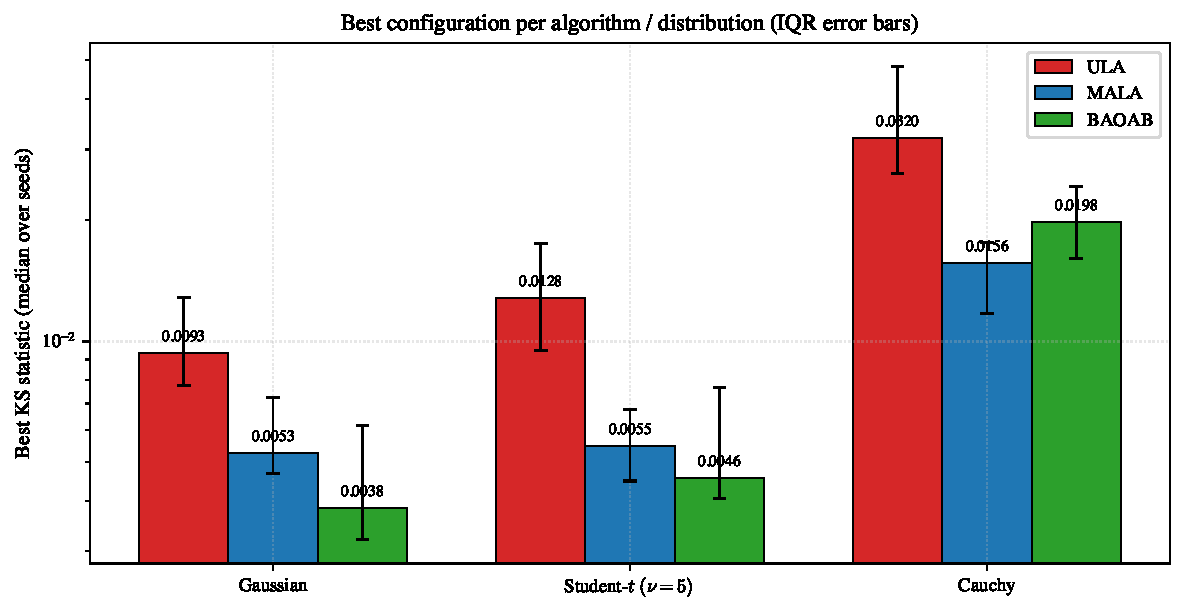
\includegraphics[width=0.85\textwidth]{../../experiments/figures/original_thesis/best_config_bars}
\caption{Καλύτερη στατιστική KS ανά αλγόριθμο σε κάθε κατανομή-στόχο, με
ράβδους σφάλματος IQR. \textbf{Χαμηλότερες τιμές είναι καλύτερες}. Ο BAOAB και ο MALA
είναι παρόμοιοι στη Γκαουσιανή και τη Student-$t$. Στην Cauchy, ο MALA
επιτυγχάνει τη χαμηλότερη KS, αλλά το χάσμα μεταξύ MALA και BAOAB είναι πολύ
μικρότερο από το χάσμα μεταξύ οποιουδήποτε εξ αυτών και του ULA.}
\label{fig:best-bars}
\end{figure}

Η κύρια κατάταξη που προκύπτει από τον Πίνακα~\ref{tab:best-configs} είναι:

\begin{itemize}
  \item Στη Γκαουσιανή και τη Student-$t$, ο BAOAB επιτυγχάνει τη χαμηλότερη διάμεσο KS ($0.0041$ και $0.0046$ αντίστοιχα), με τον MALA σε κοντινή δεύτερη θέση ($0.0056$ και $0.0055$). Η διαφορά μεταξύ BAOAB και MALA είναι αρκετά μικρή ώστε να εμπίπτει εντός της μεταβλητότητας μεταξύ εκτελέσεων.
  \item Στην Cauchy, ο MALA επιτυγχάνει τη χαμηλότερη διάμεσο KS ($0.0156$). Ο BAOAB καταλαμβάνει τη δεύτερη θέση ($0.0198$) και ο ULA την τρίτη με μεγάλη απόσταση ($0.0320$).
  \item Ο ULA είναι ο χειρότερος δειγματολήπτης σε κάθε κατανομή-στόχο. Η καλύτερη KS του είναι περίπου διπλάσια από εκείνες του MALA και του BAOAB στη Γκαουσιανή και τη Student-$t$, ενώ το χάσμα διευρύνεται περαιτέρω στην Cauchy.
\end{itemize}

Και οι δύο κύριες στρατηγικές διόρθωσης --- ο έλεγχος Metropolis στον MALA και ο
splitting ολοκληρωτής στον BAOAB --- παρέχουν ουσιαστικές βελτιώσεις έναντι της
απλής διακριτοποίησης Euler--Maruyama του ULA, ενώ η σχετική κατάταξη μεταξύ
MALA και BAOAB εξαρτάται από τη βαρύτητα ουράς της κατανομής-στόχου.

\subsection{Ετυμηγορία ανά Αλγόριθμο}

\paragraph{ULA --- μόνιμη μεροληψία σε κάθε κατανομή-στόχο.}
Ο ULA επιτυγχάνει τη βέλτιστη KS για τη Γκαουσιανή στο $\eta=0.05$, με διάμεσο
$0.0093$, περίπου διπλάσια από εκείνη του MALA ή του BAOAB. Η μεροληψία είναι
ορατή ακόμη και όταν η αλυσίδα αναμειγνύεται καλά: στο $\eta=0.05, d=1$ η
αυτοσυσχέτιση σε υστέρηση-100 είναι ουσιαστικά μηδέν για τη Γκαουσιανή, οπότε
η αλυσίδα εξερευνά το support --- απλώς εξερευνά ένα ελαφρώς \emph{λανθασμένο}
support. Αυτό δείχνει στην πράξη τη μόνιμη μεροληψία $\mathcal{O}(\eta)$ του ULA
που συζητείται στο Κεφάλαιο~\ref{chap:algorithms}.

Η μεροληψία επιδεινώνεται καθώς αυξάνεται η βαρύτητα ουράς. Για τη Student-$t$ η
βέλτιστη KS του ULA ανεβαίνει σε $0.0128$. Για την Cauchy ανεβαίνει περαιτέρω
σε $0.0320$. Η συμπεριφορά κάλυψης ουράς σε σταθερό βήμα $\eta=0.10$
τεκμηριώνεται στην Ενότητα~\ref{sec:tail-correlation} και αποτελεί τον κεντρικό
τρόπο αποτυχίας του ULA στη μελέτη αυτή.

\paragraph{MALA --- ο πιο αποδοτικός δειγματολήπτης σε ελαφριές και μέτριες ουρές.
Ο πιο ακριβής σε βαριές ουρές.}
Ο MALA επιτυγχάνει το υψηλότερο ESS στο σύνολο της μελέτης --- $36{,}047$
αποτελεσματικά δείγματα από $45{,}000$ για τη Γκαουσιανή στο $d=1$, που
αντιστοιχεί σε λόγο ESS ανά επανάληψη $0.80$, πλησίον της αναλογίας που
επιτυγχάνεται με πραγματικά ανεξάρτητα δείγματα. Τα ποσοστά αποδοχής βρίσκονται
στο εύρος $[0.78, 0.83]$ στις βέλτιστες διαμορφώσεις για τη Γκαουσιανή και τη
Student-$t$. Στην Cauchy το βέλτιστο μετατοπίζεται σε μεγαλύτερο βήμα ($\eta=4.0$)
με το ποσοστό αποδοχής να πέφτει στο $0.52$.

Το ποσοστό αποδοχής μειώνεται τόσο με τη διάσταση όσο και με τη βαρύτητα ουράς.
Στο $d=10$ για την Cauchy, η διάμεση αποδοχή στο $\eta=0.5$ είναι $0.78$, ενώ
στο $\eta=4.0$ είναι $0.49$. Αντιδιαισθητικά, για οποιοδήποτε κοινό βήμα ο
MALA αποδέχεται \emph{συχνότερα} για τη Student-$t$ παρά για τη Γκαουσιανή
(στο $\eta=1.0$, $d=1$: $0.82$ έναντι $0.78$): οι βαριές ουρές σημαίνουν ότι η
λογαριθμική πυκνότητα είναι πιο επίπεδη και ο λόγος Metropolis λιγότερο
κεντρωμένος, οπότε οι προτάσεις απορρίπτονται λιγότερο επιθετικά.
Το Σχήμα~\ref{fig:mala-accept} απεικονίζει την πλήρη συμπεριφορά αποδοχής ως
συνάρτηση του $\eta$ και του $d$, με σκίαση της ασυμπτωτικής ζώνης αναφοράς
$[0.234, 0.574]$, της οποίας το άνω άκρο $0.574$ είναι το βέλτιστο ποσοστό
αποδοχής για τον MALA ενώ το κάτω άκρο $0.234$ αντιστοιχεί στον Random-Walk
Metropolis \citep{roberts1998optimal}. Και τα δύο όρια είναι υπερβολικά χαμηλά
για $d\le 10$ και τα εμπειρικά βέλτιστά μας βρίσκονται πάνω από αυτήν.

\begin{figure}[ht]
\centering
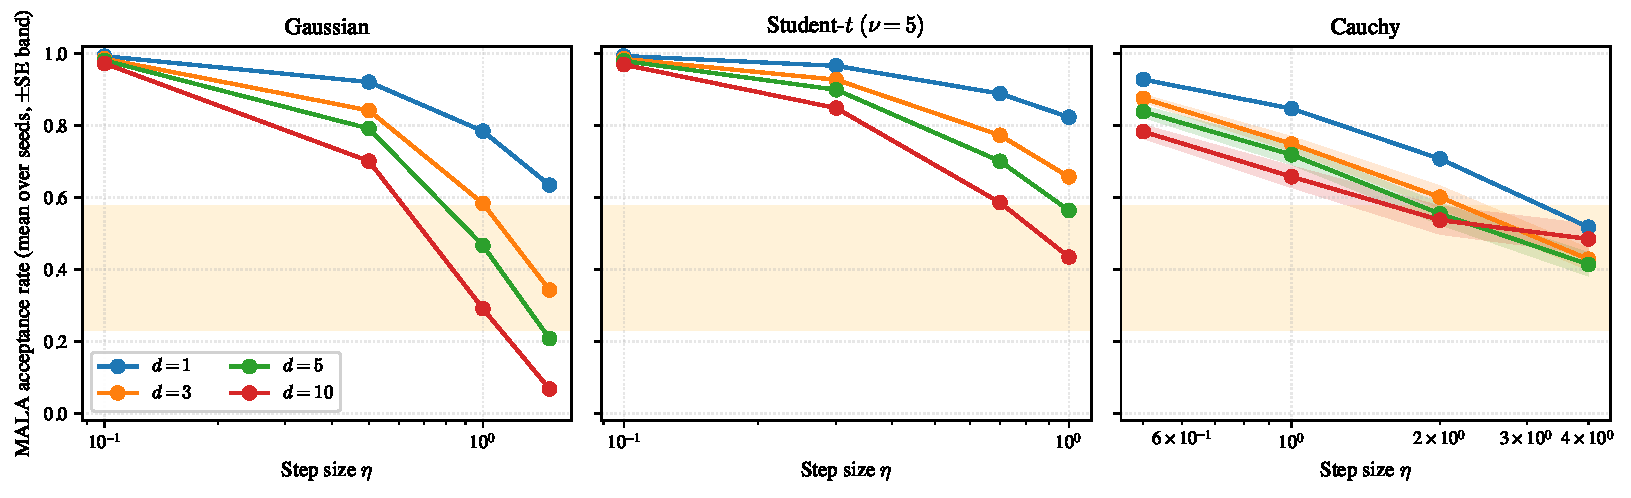
\includegraphics[width=\textwidth]{../../experiments/figures/original_thesis/mala_acceptance}
\caption{Ποσοστό αποδοχής του MALA ως συνάρτηση του βήματος και της διάστασης,
στις τρεις κατανομές-στόχους. Κάθε γραμμή είναι ο μέσος μεταξύ $20$ εκτελέσεων με
ζώνη σκίασης $\pm$ τυπικό σφάλμα. Οι γραμμές χρωματίζονται ανά διάσταση. Η
πορτοκαλί ζώνη σηματοδοτεί την ασυμπτωτική περιοχή αναφοράς $[0.234, 0.574]$
(άνω άκρο $0.574$ = βέλτιστο MALA, κάτω άκρο $0.234$ = βέλτιστο Random-Walk
Metropolis).}
\label{fig:mala-accept}
\end{figure}

\paragraph{BAOAB --- H μικρότερη απόκλιση σε ελαφριές ουρές στο $d=1$,
με τις μικρότερες μεροληψίες ροπών.}
Ο BAOAB επιτυγχάνει τη χαμηλότερη διάμεσο KS στο $d=1$ για τη Γκαουσιανή
($0.0041$) και τη Student-$t$ ($0.0046$), υπερτερώντας οριακά του MALA και στις
δύο περιπτώσεις. Το πλεονέκτημα έναντι του MALA είναι της τάξης $25$--$50\%$
στο KS στατιστικό. Το ESS στο $d=1$ είναι περίπου το μισό εκείνου του MALA για τη Γκαουσιανή ($20{,}500$ έναντι $36{,}000$). Ο BAOAB δεν έχει απορριπτόμενες προτάσεις αλλά απαιτεί δύο
αξιολογήσεις κλίσης ανά βήμα αντί για μία συν μία αξιολόγηση λογαριθμικής
πυκνότητας, οπότε η σύγκριση ως προς χρόνο εκτέλεσης είναι πιο κοντινή από
ό,τι υποδηλώνει η διαφορά ESS.

Επιπλέον, ο BAOAB παράγει τις μικρότερες μεροληψίες ροπών από τους τρεις
αλγορίθμους στη Γκαουσιανή και τη Student-$t$ κατανομή-στόχο. Στο $d=1$ για
τη Γκαουσιανή, η απόλυτη μεροληψία του εκτιμητή μέσου είναι $0.001$ και του
εκτιμητή διακύμανσης $0.0003$ --- περίπου πέντε φορές μικρότερες από τις
μεροληψίες του MALA για τον ίδιο στόχο. Το σφάλμα διακριτοποίησης του BAOAB
ολοκληρωτή είναι ανώτερης τάξης από εκείνο του ULA, κάτι που εκδηλώνεται σε
αυτού του είδους τη λεπτομερή σύγκριση ακρίβειας.

Η δομικά σημαντική ιδιότητα του BAOAB --- ότι η KS του για τη Γκαουσιανή
κατανομή-στόχο παραμένει περίπου σταθερή καθώς αυξάνεται η διάσταση ---
αναλύεται στην Ενότητα~\ref{sec:dim-scaling}, όπου ο πίνακας κλιμάκωσης
διάστασης καθιστά ρητή τη σύγκριση με τον MALA.

\subsection{Ευαισθησία στην Παράμετρο Τριβής $\gamma$ του BAOAB}
\label{sec:gamma-sensitivity}

Ο BAOAB ολοκληρωτής εξαρτάται από μια παράμετρο τριβής $\gamma$ που ελέγχει
πόσο γρήγορα αποσβένεται η ορμή. Μικρό $\gamma$ επιτρέπει στην ορμή να
συσσωρεύεται μεταξύ βημάτων. Μεγάλο $\gamma$
αναγκάζει την ορμή να αποκαθίσταται γρήγορα (καθεστώς διαχυτικής κίνησης, εμφανίζοντας παρόμοια συμπεριφορά με τον ULA).

Λαμβάνοντας μέσο όρο επί των διαμορφώσεων $(\eta, d)$, η μέση KS βελτιώνεται
μονότονα για μικρό $\gamma$ σε κάθε κατανομή-στόχο:

\begin{table}[ht]
\centering
\small
\begin{tabular}{lcccc}
\toprule
                & $\gamma = 0.5$ & $\gamma = 1.0$ & $\gamma = 2.0$ & $\gamma = 5.0$ \\
\midrule
Γκαουσιανή KS     & $0.0064$ & $0.0072$ & $0.0084$ & $0.0110$ \\
Student-$t$ KS  & $0.0081$ & $0.0088$ & $0.0101$ & $0.0134$ \\
Cauchy KS       & $0.0421$ & $0.0498$ & $0.0596$ & $0.0830$ \\
\bottomrule
\end{tabular}
\caption{Μέση KS επί των διαμορφώσεων $(\eta, d)$, ανά τιμή τριβής $\gamma$.
Σε κάθε κατανομή-στόχο η διάμεση KS βελτιώνεται ομαλά καθώς το $\gamma$
μειώνεται.}
\label{tab:gamma-mean}
\end{table}

Ο κανόνας «μικρό $\gamma$ είναι καλύτερο» ισχύει στο επίπεδο της διαμέσου KS
κατά μέσο όρο ως προς τις υπερπαραμέτρους. Σε επίπεδο μεμονωμένων βέλτιστων
διαμορφώσεων η εικόνα είναι λιγότερο ξεκάθαρη: για τον BAOAB στη Γκαουσιανή
στο $d=1, \eta=1.0$, και οι τέσσερις τιμές $\gamma$ παράγουν στατιστικώς
αδιάκριτες διαμέσους KS (οι τέσσερις διάμεσοι καλύπτουν μόνο το διάστημα
$0.0038$--$0.0041$, καλά εντός του IQR της καθεμίας). Αυτό που τις διαφοροποιεί
σε αυτή τη βέλτιστη διαμόρφωση είναι το ESS: το $\gamma=0.5$ παρέχει $20{,}498$
αποτελεσματικά δείγματα έναντι $11{,}865$ στο $\gamma=5.0$, βελτίωση $70\%$.
Με άλλα λόγια, η χαμηλή τριβή είναι η ασφαλής επιλογή όταν δεν είναι εφικτή
ακριβής ρύθμιση εκ των προτέρων. Το Σχήμα~\ref{fig:baoab-gamma} απεικονίζει
αυτήν την τάση.

\begin{figure}[ht]
\centering
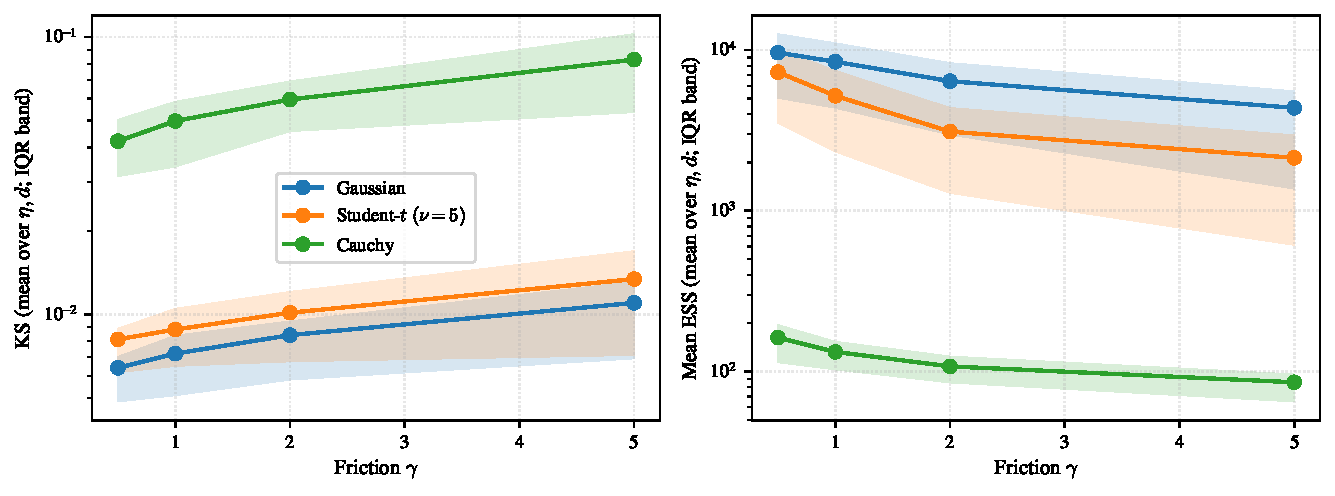
\includegraphics[width=\textwidth]{../../experiments/figures/original_thesis/baoab_gamma_sensitivity}
\caption{Ευαισθησία του BAOAB στην παράμετρο τριβής $\gamma$ στις τρεις
κατανομές-στόχους, με ζώνες σφάλματος IQR. Τόσο το πλαίσιο KS (αριστερά) όσο
και το πλαίσιο ESS (δεξιά) ευνοούν μικρό $\gamma$ κατά μέσο όρο επί του
πλέγματος υπερπαραμέτρων.}
\label{fig:baoab-gamma}
\end{figure}

Αυτό το εμπειρικό μοτίβο αντιφάσκει με μια κοινή εγχειριδιακή διαίσθηση ότι
οι βαρύτερες ουρές ωφελούνται από \emph{περισσότερη} τριβή \citep{leimkuhler2015molecular} (επειδή η αλυσίδα
χρειάζεται να αποσβεστεί ενάντια στις μακρές εκδρομές). Τα εμπειρικά δεδομένα
είναι αναμφίβολα: και στις τρεις κατανομές-στόχους, η χαμηλή τριβή κερδίζει
κατά μέσο όρο, τόσο στην KS όσο και στο ESS.

\subsection{Κλιμάκωση ως προς τη Διάσταση}
\label{sec:dim-scaling}

Επεκτείνουμε το πλέγμα από $d \in \{1, 3, 5, 10\}$ σε
$d \in \{20, 50, 100\}$ και εξετάζουμε εκ νέου τη μέση KS ανά αλγόριθμο σε
κάθε διάσταση. Το κεντρικό αποτέλεσμα, ορατό στον
Πίνακα~\ref{tab:dim-scaling-numbers} παρακάτω, είναι ότι \emph{η KS του BAOAB
για τη Γκαουσιανή κατανομή-στόχο είναι ουσιαστικά σταθερή σε ολόκληρο το
εξεταζόμενο εύρος διαστάσεων}. Η τιμή του KS στις 100 διαστάσεις (0.006) διαφέρει ελάχιστα από την αντίστοιχη της μίας διάστασης (0.007). Σε σύγκριση, η μέση KS του MALA για τη Γκαουσιανή αυξάνεται κατά παράγοντα $15$ στο ίδιο εύρος (από
$0.007$ σε $0.109$). Αυτό αποτελεί το ισχυρότερο εμπειρικό τεκμήριο υπέρ του underdamped σχήματος όσον αφορά τη συμπεριφορά του σε υψηλές
διαστάσεις για λογαριθμικά-κυρτές κατανομές-στόχους.

Το Σχήμα~\ref{fig:dim-scaling} απεικονίζει τη μέση KS ως συνάρτηση της
διάστασης για $d \in \{1, 3, 5, 10, 20, 50, 100\}$, κατά μέσο όρο επί των
διαμορφώσεων $(\eta, \gamma)$. Ο Πίνακας~\ref{tab:dim-scaling-numbers} παρέχει
τις υποκείμενες αριθμητικές τιμές.

\begin{table}[ht]
\centering
\small
\begin{tabular}{llccccccc}
\toprule
Αλγ. & Κατανομή & $d{=}1$ & $d{=}3$ & $d{=}5$ & $d{=}10$ & $d{=}20$ & $d{=}50$ & $d{=}100$ \\
\midrule
ULA   & Γκαουσιανή    & $0.015$ & $0.018$ & $0.020$ & $0.020$ & $0.021$ & $0.021$ & $0.020$ \\
ULA   & Student-$t$ & $0.026$ & $0.031$ & $0.035$ & $0.045$ & $0.034$ & $0.045$ & $0.064$ \\
ULA   & Cauchy      & $0.042$ & $0.060$ & $0.065$ & $0.096$ & $0.258$ & $0.599$ & $0.640$ \\
MALA  & Γκαουσιανή    & $0.007$ & $0.008$ & $0.010$ & $0.015$ & $0.012$ & $0.040$ & $0.109$ \\
MALA  & Student-$t$ & $0.008$ & $0.008$ & $0.010$ & $0.012$ & $0.016$ & $0.031$ & $0.031$ \\
MALA  & Cauchy      & $0.020$ & $0.029$ & $0.049$ & $0.074$ & $0.080$ & $0.348$ & $0.593$ \\
BAOAB & Γκαουσιανή    & $0.007$ & $0.008$ & $0.009$ & $0.009$ & $0.006$ & $0.006$ & $0.006$ \\
BAOAB & Student-$t$ & $0.008$ & $0.010$ & $0.010$ & $0.011$ & $0.012$ & $0.012$ & $0.013$ \\
BAOAB & Cauchy      & $0.042$ & $0.056$ & $0.061$ & $0.075$ & $0.125$ & $0.497$ & $0.566$ \\
\bottomrule
\end{tabular}
\caption{Μέσος της διαμέσου KS επί των διαμορφώσεων $(\eta, \gamma)$, ανά ζεύγος
(αλγόριθμος, κατανομή, διάσταση). Οι κατανομές-στόχοι Γκαουσιανή και Student-$t$
υποβαθμίζονται αργά με τη διάσταση και για τους τρεις αλγορίθμους. Η κατανομή
Cauchy υποβαθμίζεται σοβαρά και για τους τρεις, ιδίως πέραν του $d = 10$.
Σημειώστε τη στήλη Γκαουσιανής του BAOAB: η KS παραμένει στο $\approx 0.006$
ως και το $d = 100$.}
\label{tab:dim-scaling-numbers}
\end{table}

Τρία μοτίβα είναι ορατά:

\begin{itemize}
\item \textbf{Για τη Γκαουσιανή κατανομή-στόχο}, και οι τρεις αλγόριθμοι
      παραμένουν σταθεροί έως το $d = 100$, με αμετάβλητη σειρά αξίας. Η KS
      του BAOAB είναι ουσιαστικά σταθερή στο $\approx 0.006$ σε ολόκληρο το
      εξεταζόμενο εύρος διαστάσεων --- η ανθεκτικότητα ως προς τη διάσταση του
      underdamped σχήματος είναι εντυπωσιακή. Ο MALA υποβαθμίζεται πιο εμφανώς
      σε υψηλό $d$ (από $0.007$ στο $d=1$ σε $0.109$ στο $d=100$), καθώς το
      ποσοστό αποδοχής του κινείται προς το ασυμπτωτικό καθεστώς
      Roberts--Rosenthal που συζητείται στην Ενότητα~\ref{sec:grid-study}.
\item \textbf{Για τη Student-$t$ κατανομή-στόχο}, και οι τρεις αλγόριθμοι
      παραμένουν εύλογοι σε ολόκληρο το εύρος. Η μεροληψία του ULA αυξάνεται με
      τη διάσταση ($0.026 \to 0.064$). Η KS του MALA αυξάνεται παρόμοια. Ο BAOAB
      παρακολουθεί στενά τον MALA καθ' όλη τη διάρκεια.
\item \textbf{Για τη Cauchy κατανομή-στόχο}, και οι τρεις αλγόριθμοι
      υποβαθμίζονται σοβαρά πέραν του $d = 10$, και στο $d = 100$ οι μέσες
      τιμές KS και των τριών είναι πάνω από $0.5$ --- λειτουργικά, κανένας από
      αυτούς δεν δειγματίζει την κατανομή-στόχο στο $d = 100$. Η πτώση είναι
      πιο απότομη μεταξύ $d = 10$ και $d = 50$. Στο $d = 100$ οι τρεις
      αλγόριθμοι είναι ουσιαστικά ισόπαλοι σε επίπεδο αποτυχίας. Αυτή είναι η
      σημαντικότερη εμπειρική παρατήρηση σχετικά με τη δειγματοληψία βαριών
      ουρών σε αυτή την εργασία: η δυσκολία δεν κλιμακώνεται ήπια με τη
      διάσταση αλλά αλλάζει το καθεστώς κάπου στο $20 \le d \le 50$.
\end{itemize}

Αξίζει επίσης να σημειωθεί ότι η αναλογία ESS του BAOAB για τη Γκαουσιανή
παραμένει σταθερή ανεξάρτητα από τη διάσταση. Το μέσο ESS μεταξύ διαμορφώσεων στο $d=1$ είναι
περίπου $9{,}600$ και στο $d=10$ περίπου $4{,}500$. Στο $d = 100$ παραμένει
πάνω από $1{,}000$, μια αργή λογαριθμική πτώση αντί της πτώσης κατά παράγοντα
πέντε ανά δεκάδα που εκδηλώνει ο MALA στο ίδιο εύρος. Αυτό δείχνει στην πράξη γιατί τα underdamped σχήματα έχουν προσελκύσει τόσο
ενδιαφέρον στη σύγχρονη βιβλιογραφία για kinetic δειγματολήπτες Langevin
\citep{cheng2018underdamped, leimkuhler2015molecular, neal2011mcmc}, και
ισχύει έως τις μεγαλύτερες διαστάσεις που δοκιμάσαμε.

\begin{figure}[ht]
\centering
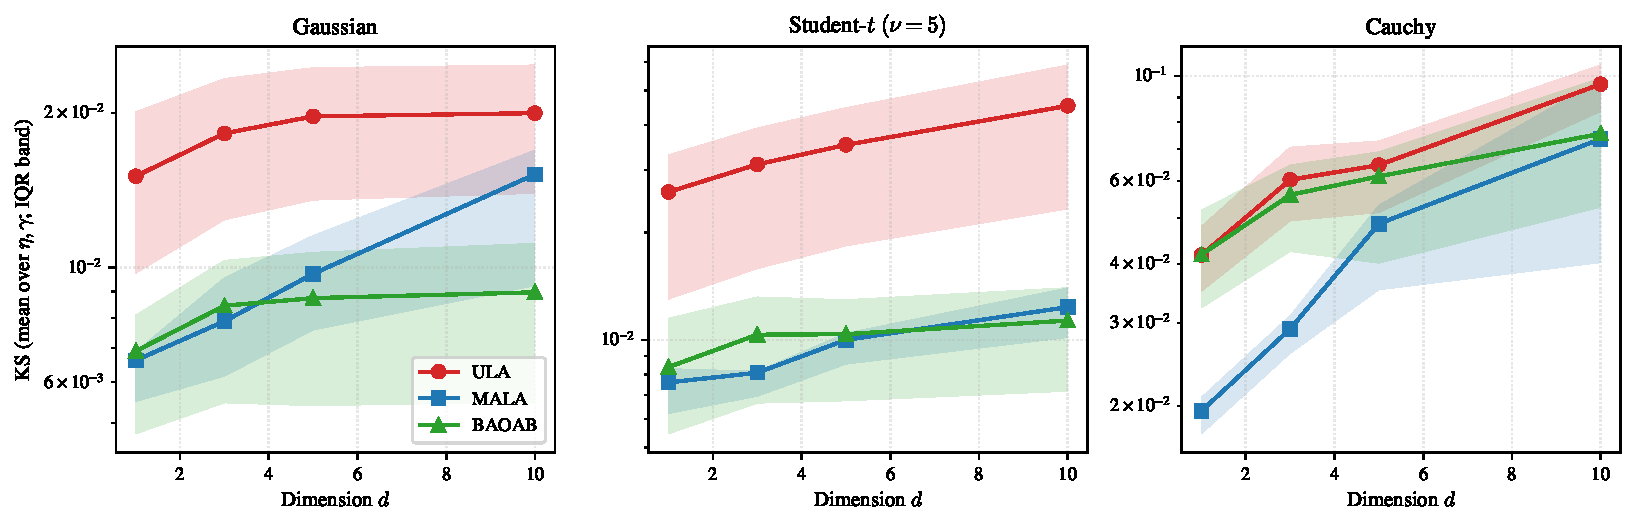
\includegraphics[width=\textwidth]{../../experiments/figures/original_thesis/dimension_scaling_ks}
\caption{KS ως συνάρτηση της διάστασης, κατά μέσο όρο επί του
πλέγματος $(\eta, \gamma)$ για κάθε αλγόριθμο. Η σκιασμένη ζώνη δείχνει το
διατεταρτημοριακό εύρος των διαμέσων ανά διαμόρφωση. Και οι δύο άξονες είναι
σε λογαριθμική κλίμακα.}
\label{fig:dim-scaling}
\end{figure}

\subsection{Κόστος Χρόνου Εκτέλεσης}
\label{sec:exec-time}

Το κόστος ανά επανάληψη κάθε δειγματολήπτη διαφέρει: ο ULA εκτελεί μία
αξιολόγηση κλίσης ανά βήμα. Ο MALA εκτελεί μία αξιολόγηση κλίσης και μία
αξιολόγηση λογαριθμικής πυκνότητας, συν έναν έλεγχο αποδοχής/απόρριψης. Ο
BAOAB εκτελεί δύο αξιολογήσεις κλίσης ανά βήμα στις ενημερώσεις μισής δύναμης
και δεν έχει έλεγχο αποδοχής/απόρριψης. Αν αυτές οι διαφορές ανά βήμα
μεταφράζονται σε χρήσιμες διαφορές χρόνου εκτέλεσης εξαρτάται από την
υλοποίηση, το κόστος κλίσης της κατανομής-στόχου και τη διάσταση. Ο
Πίνακας~\ref{tab:runtime-cost} παρέχει τους εμπειρικούς αριθμούς στο $d=1$ για
κάθε κατανομή-στόχο, μετρημένους στην υλοποίησή μας που χρησιμοποιεί τα πακέτα NumPy/SciPy. Το ESS ανά δευτερόλεπτο συνδυάζει χρόνο εκτέλεσης και αποτελεσματικό
μέγεθος δείγματος και αποτελεί την τυπική μετρική αποδοτικότητας προσαρμοσμένης
ως προς το κόστος για MCMC.

\begin{table}[H]
\centering
\small
\begin{tabular}{llrrr}
\toprule
Αλγόριθμος & Κατανομή-στόχος & Χρόνος εκτέλεσης (s) & ESS & ESS / sec \\
\midrule
ULA   & Γκαουσιανή    & $0.14$ & $1{,}205$  & $\phantom{0}8{,}600$ \\
ULA   & Student-$t$ & $0.27$ & $\phantom{1}608$    & $\phantom{0}2{,}250$ \\
ULA   & Cauchy      & $0.25$ & $\phantom{1}124$    & $\phantom{0}\phantom{0}495$ \\
MALA  & Γκαουσιανή    & $0.60$ & $16{,}900$ & $28{,}000$ \\
MALA  & Student-$t$ & $1.10$ & $12{,}800$ & $11{,}550$ \\
MALA  & Cauchy      & $1.01$ & $\phantom{1}576$    & $\phantom{0}\phantom{0}563$ \\
BAOAB & Γκαουσιανή    & $0.35$ & $14{,}800$ & $41{,}900$ \\
BAOAB & Student-$t$ & $0.64$ & $\phantom{1}6{,}800$  & $10{,}600$ \\
BAOAB & Cauchy      & $0.58$ & $\phantom{1}262$    & $\phantom{0}\phantom{0}453$ \\
\bottomrule
\end{tabular}
\caption{Χρόνος εκτέλεσης ανά αλυσίδα και αποδοτικότητα στο $d=1$, βέλτιστη
διαμόρφωση ανά ζεύγος (αλγόριθμος, κατανομή-στόχος). Ο χρόνος εκτέλεσης είναι
ανά $5\!\times\!10^4$ επαναλήψεις, μέσος μεταξύ $20$ εκτελέσεων. Το κόστος ανά
επανάληψη του ULA είναι το χαμηλότερο αλλά το χαμηλό ESS του δίνει το χειρότερο
ESS ανά δευτερόλεπτο. Ο BAOAB και ο MALA βρίσκονται εντός παράγοντα $1.5$ στο
ESS ανά δευτερόλεπτο για τη Γκαουσιανή και τη Student-$t$ στο $d=1$. Στην Cauchy
και οι τρεις αλγόριθμοι περιορίζονται από το χαμηλό τους ESS παρά από το κόστος
ανά επανάληψη.}
\label{tab:runtime-cost}
\end{table}

Η εικόνα στο $d=1$ είναι ότι \textbf{ο MALA και ο BAOAB είναι συγκρίσιμοι σε
αποδοτικότητα χρόνου εκτέλεσης για τη Γκαουσιανή και τη Student-$t$
κατανομή-στόχο}, με τον BAOAB περίπου $50\%$ μπροστά για τη Γκαουσιανή και τον
MALA περίπου $10\%$ μπροστά για τη Student-$t$. Το χάσμα κλείνει περαιτέρω στην
Cauchy, όπου και οι τρεις αλγόριθμοι παράγουν τόσο λίγο ESS ανά αλυσίδα ώστε
ο χρόνος-ρολογιού ανά ESS να κυριαρχείται από τη δυσκολία της κατανομής-στόχου
παρά από την επιβάρυνση οποιουδήποτε αλγορίθμου.

Η εικόνα αλλάζει δραματικά καθώς η διάσταση αυξάνεται.
Το Σχήμα~\ref{fig:ess-per-sec} απεικονίζει το ESS ανά δευτερόλεπτο ως συνάρτηση
της διάστασης στη βέλτιστη διαμόρφωση ανά αλγόριθμο για τη Γκαουσιανή
κατανομή-στόχο.

\begin{figure}[H]
\centering
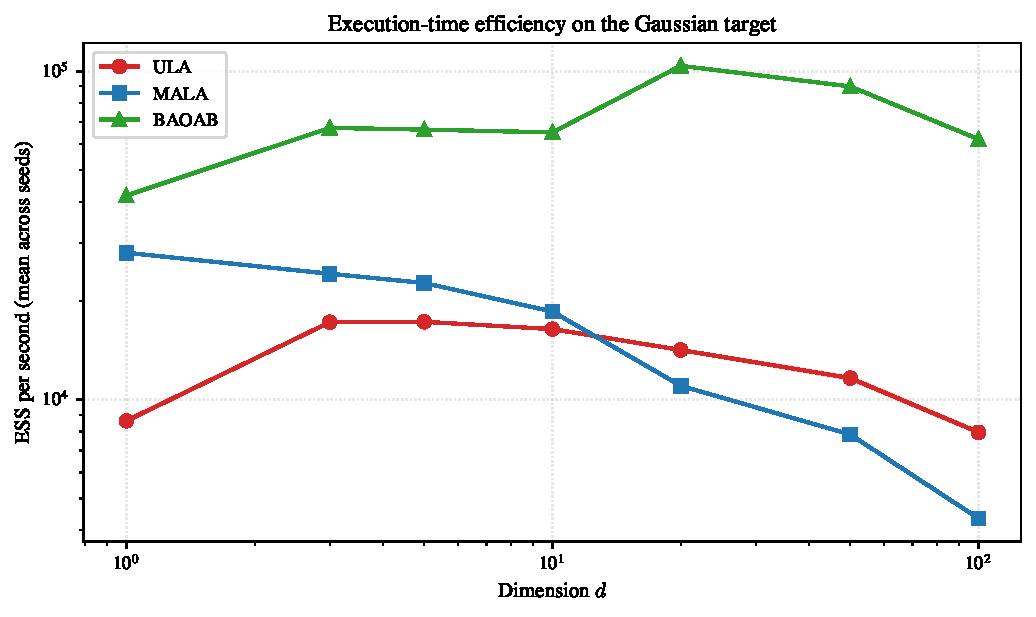
\includegraphics[width=0.85\textwidth]{../../experiments/figures/original_thesis/ess_per_sec_gaussian}
\caption{ESS ανά δευτερόλεπτο ως συνάρτηση της διάστασης στη βέλτιστη διαμόρφωση
ανά αλγόριθμο για τη Γκαουσιανή κατανομή-στόχο. Και οι δύο άξονες είναι
λογαριθμικοί. Η αποδοτικότητα του BAOAB αυξάνεται με τη διάσταση έως
$d\approx 20$ και παραμένει μια τάξη μεγέθους πάνω από τον MALA στο $d=100$.}
\label{fig:ess-per-sec}
\end{figure}

Δύο χαρακτηριστικά του Σχήματος~\ref{fig:ess-per-sec} αξίζουν προσοχής.
Πρώτον, το ESS ανά δευτερόλεπτο του BAOAB για τη Γκαουσιανή \emph{αυξάνεται} με τη διάσταση, από $42{,}000$ στο $d=1$ σε κορύφωση
$104{,}000$ στο $d=20$, πριν μειωθεί αργά σε $62{,}000$ στο $d=100$. Αυτό
αντικατοπτρίζει δύο παράγοντες: η KS του BAOAB παραμένει περίπου σταθερή καθώς
αυξάνεται το $d$ (Ενότητα~\ref{sec:dim-scaling}), και το κόστος ανά επανάληψη
αυξάνεται μόνο ελαφρά με το $d$ στην υλοποίησή μας NumPy επειδή η αλυσίδα
επεξεργάζεται όλες τις συντεταγμένες σε διανυσματοποιημένες πράξεις πίνακα.
Δεύτερον, \textbf{το ESS ανά δευτερόλεπτο του MALA πέφτει απότομα με τη
διάσταση}, από $28{,}000$ στο $d=1$ σε $4{,}400$ στο $d=100$. Στο $d=10$ ο
BAOAB είναι περίπου $3.5\times$ πιο αποδοτικός από τον MALA ανά δευτερόλεπτο.
Στο $d=100$, $14\times$ πιο αποδοτικός.

Η ανθεκτικότητα του BAOAB ως προς τη διάσταση οδηγεί συνεπώς σε πολύ καλύτερη
απόδοση σε σχέση με το υπολογιστικό κόστος από ό,τι υποδηλώνει μόνη της η
σύγκριση ESS ανά επανάληψη. Η αλγοριθμική σύσταση
που προκύπτει είναι απλή: \emph{για δειγματοληψία μέτριας έως υψηλής διάστασης
σε λογαριθμικά-κυρτές κατανομές-στόχους, ο BAOAB παρέχει ουσιαστικά
περισσότερα αποτελεσματικά δείγματα ανά δευτερόλεπτο από τον MALA στην
υλοποίησή μας.}

\section{Βαρύτητα Ουράς και Μεροληψία}
\label{sec:tail-correlation}

Το κεντρικό ερώτημα της εργασίας είναι πώς οι τρεις δειγματολήπτες
ανταποκρίνονται στην αυξανόμενη βαρύτητα ουράς. Απομονώνουμε την επίδραση
καθηλώνοντας $d=1$ και $\eta=0.10$ για τον ULA --- ένα βήμα παρόν στο πλέγμα
ULA και για τις τρεις κατανομές-στόχους --- και συγκρίνουμε τι κάνει η αλυσίδα
στις τρεις κατανομές. Το Σχήμα~\ref{fig:ula-bias} δείχνει το αποτέλεσμα, και ο
Πίνακας~\ref{tab:ula-tails} συλλέγει τους υποκείμενους αριθμούς.

\begin{table}[ht]
\centering
\small
\begin{tabular}{lccccc}
\toprule
Κατανομή     & διάμεση KS              & q-MAE q=0.025 & q-MAE q=0.975 & κάλ. ουράς q=0.01 & κάλ. ουράς q=0.99 \\
\midrule
Γκαουσιανή         & $0.0099$ ($0.0080, 0.0140$)  & $0.052$ & $0.050$ & $1.17$ & $1.17$ \\
Student-$t$      & $0.0131$ ($0.0103, 0.0176$)  & $0.048$ & $0.102$ & $0.98$ & $1.02$ \\
Cauchy           & $0.0359$ ($0.0292, 0.0549$)  & $6.54$  & $5.15$  & $0.00$ & $0.00$ \\
\bottomrule
\end{tabular}
\caption{Διαγνωστικά ULA στο $\eta=0.10$, $d=1$, για τις τρεις κατανομές-στόχους.
Διάμεσος μεταξύ $20$ εκτελέσεων. IQR σε παρένθεση για τη στήλη KS. Οι αναλογίες
κάλυψης ουράς στις δύο τελευταίες στήλες θα έπρεπε να είναι $1.0$ σε έναν
ιδανικά συμπεριφερόμενο δειγματολήπτη.}
\label{tab:ula-tails}
\end{table}

\begin{figure}[ht]
\centering
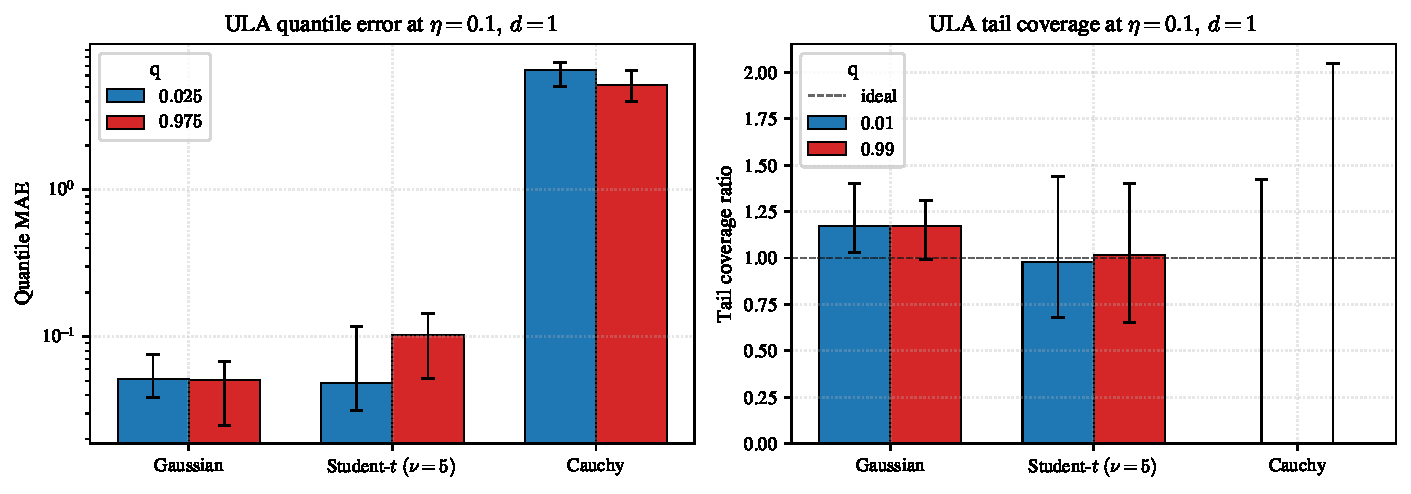
\includegraphics[width=\textwidth]{../../experiments/figures/original_thesis/ula_bias_inversion}
\caption{ULA στο ίδιο βήμα για τις τρεις κατανομές-στόχους. Αριστερά: σφάλμα
στα εμπειρικά ποσοστημόρια $2.5\%$ και $97.5\%$, με ράβδους σφάλματος IQR σε
λογαριθμική κλίμακα. Δεξιά: αναλογίες κάλυψης ουράς στο $1\%$ και $99\%$.
Η οριζόντια γραμμή δείχνει την ιδανική τιμή $1.0$.}
\label{fig:ula-bias}
\end{figure}

Διακρίνονται τρία διακριτά καθεστώτα αποτυχίας:

\begin{enumerate}
  \item \textbf{Γκαουσιανή (ελαφριές ουρές):} ο ULA \emph{υπερ-καλύπτει} τις
        ουρές κατά περίπου $17\%$ (αναλογία κάλυψης ουράς $1.17$). Η αλυσίδα
        τοποθετεί ελαφρώς περισσότερη μάζα πέραν του θεωρητικού ποσοστημορίου
        $99\%$ από ό,τι έπρεπε. Τα εμπειρικά ακραία ποσοστημόρια είναι ήπια
        υπερβολικά ακραία. Τα σφάλματα ποσοστημορίου στα επίπεδα $2.5\%/97.5\%$
        είναι της τάξης $0.05$ --- μικρά σε απόλυτους όρους αλλά ορατά.
  \item \textbf{Student-$t$ (μέτριες ουρές):} η υπερ-κάλυψη της Γκαουσιανής
        εξαφανίζεται και οι αναλογίες κάλυψης ουράς είναι ουσιαστικά μοναδιαίες.
        Το σφάλμα ποσοστημορίου στο άνω άκρο διπλασιάζεται ($0.05 \to 0.10$) ---
        η αλυσίδα έχει περίπου το σωστό σχήμα αλλά τα εμπειρικά ακραία
        ποσοστημόρια είναι πιο θορυβώδη.
  \item \textbf{Cauchy (βαριές ουρές):} ο τρόπος μεροληψίας \emph{αντιστρέφεται}.
        Αντί να υπερ-καλύπτει τις ουρές, η αλυσίδα αποτυγχάνει να τις φτάσει. Η αναλογία κάλυψης ουράς στο $q=0.01$ και $q=0.99$ καταρρέει
        σε μηδέν σε κάθε μία από τις $20$ εκτελέσεις. Το σφάλμα ποσοστημορίου
        στο επίπεδο $97.5\%$ εκτοξεύεται από $0.05$ (Γκαουσιανή) σε $0.10$
        (Student-$t$) σε $5.15$ (Cauchy), μία εκατονταπλάσια αύξηση.
\end{enumerate}

Ο μηχανισμός είναι γεωμετρικός. Το βήμα πρότασης του ULA είναι
$-\eta \nabla U(X) + \sqrt{2\eta}\,\xi$. Για τη Γκαουσιανή, $\nabla U(x) = x$,
οπότε η ντετερμινιστική ολίσθηση πάντοτε επαναφέρει την αλυσίδα προς την αρχή
με δύναμη ανάλογη του $\|x\|$. Για την Cauchy, η κλίση είναι
$\nabla U(x) = (d+1) x / (1+\|x\|^2)$, η οποία τείνει \emph{στο μηδέν} καθώς
$\|x\|\to\infty$. Μόλις μια αλυσίδα Cauchy βρεθεί μακριά από την αρχή, δεν
υπάρχει ντετερμινιστική επαναφορική δύναμη, και ο μόνος μηχανισμός για να
παραμείνει στην ουρά ή να την αφήσει είναι ο όρος θορύβου, που έχει αναμενόμενο
μέγεθος $\sqrt{2\eta} \approx 0.45$ --- πολύ μικρότερο από το θεωρητικό
ποσοστημόριο $99\%$ της Cauchy στο $\pm 31.8$. Η αλυσίδα αδυνατεί να πραγματοποιήσει άλμα από την αρχή
στο $\pm 30$ σε πεπερασμένο χρόνο, ούτε, έχοντας φτάσει σε τέτοια περιοχή,
να επιστρέψει από αυτήν αποδοτικά.

Ο MALA αντισταθμίζει εν μέρει επιτρέποντας μεγαλύτερα βήματα (το βέλτιστο
$\eta$ για τον MALA στην Cauchy είναι $4.0$, οκτώ φορές μεγαλύτερο από εκείνο
του ULA), αλλά το ποσοστό αποδοχής Metropolis μειώνεται αντίστοιχα. Ο BAOAB
παρακάμπτει το πρόβλημα διαφορετικά --- η ενημέρωση Ornstein--Uhlenbeck στη μεταβλητή ταχύτητας επιτρέπει στην αλυσίδα
να κινείται προς μακρινές περιοχές με τη βοήθεια της ορμής, χωρίς να χρειάζεται
μια μεμονωμένη μεγάλη πρόταση.
Τεκμηριώνουμε τις συνέπειες στη μελέτη σύγκλισης
(Ενότητα~\ref{sec:convergence-study}) και στις μελέτες περίπτωσης που ακολουθούν.

\subsection{Εξάρτηση από τη Διάσταση των Ευρημάτων Ουράς}
\label{sec:dim-dependence-tails}

Το κεντρικό εύρημα αυτής της υποενότητας είναι μια \emph{αλλαγή καθεστώτος}
στη δειγματοληψία Cauchy μεταξύ $d=10$ και $d=50$. Κάτω από $d=10$ και οι τρεις
αλγόριθμοι διαχειρίζονται την Cauchy με μεταβλητό βαθμό επιτυχίας (μέση KS
βέλτιστης διαμόρφωσης στο $[0.02, 0.10]$). Στο $d=100$ και οι τρεις
αποτυγχάνουν λειτουργικά, με μέση KS πάνω από $0.5$ για κάθε αλγόριθμο. Η
κατάρρευση δεν είναι ομαλή υποβάθμιση: μεταξύ $d=10$ και $d=50$ η μέση KS
αυξάνεται κατά παράγοντα πέντε για κάθε αλγόριθμο, και πέραν του $d=50$ οι
διαφορές μεταξύ αλγορίθμων εξαφανίζονται. Πρόκειται για γεωμετρική ιδιότητα των
κατανομών βαριάς ουράς σε υψηλή διάσταση --- το τυπικό σύνολο μιας Cauchy στο
$\mathbb{R}^d$ μετακινείται προς τα έξω με $d$ ταχύτερα από ό,τι μπορεί να
ακολουθήσει οποιοσδήποτε δειγματολήπτης βασισμένος σε κλίση --- και δεν είναι πρόβλημα κάποιου συγκεκριμένου αλγορίθμου, αλλά
γεωμετρία των βαριών ουρών σε υψηλή διάσταση.

Η ποιοτική συμπεριφορά που μόλις περιγράφηκε --- πώς ο ULA αντιστρέφει την
μεροληψία, ο MALA αντισταθμίζει μεγεθύνοντας το βήμα, και ο BAOAB εκμεταλλεύεται
την ορμή --- είναι γεωμετρικά αναπόφευκτη σε κάθε διάσταση. Το εμπειρικό ερώτημα είναι πόσο
γρήγορα η δυσκολία αυξάνεται με $d$. Το Σχήμα~\ref{fig:cauchy-dim} απεικονίζει
τρία διαγνωστικά Cauchy --- την προσαρμογή κορμού (KS), το σφάλμα ακραίου
ποσοστημορίου (q-MAE στο $q=0.975$) και την αναλογία κάλυψης άνω ουράς --- ως
συνάρτηση της διάστασης για τη βέλτιστη διαμόρφωση κάθε αλγορίθμου σε εκείνη
τη διάσταση.

\begin{figure}[ht]
\centering
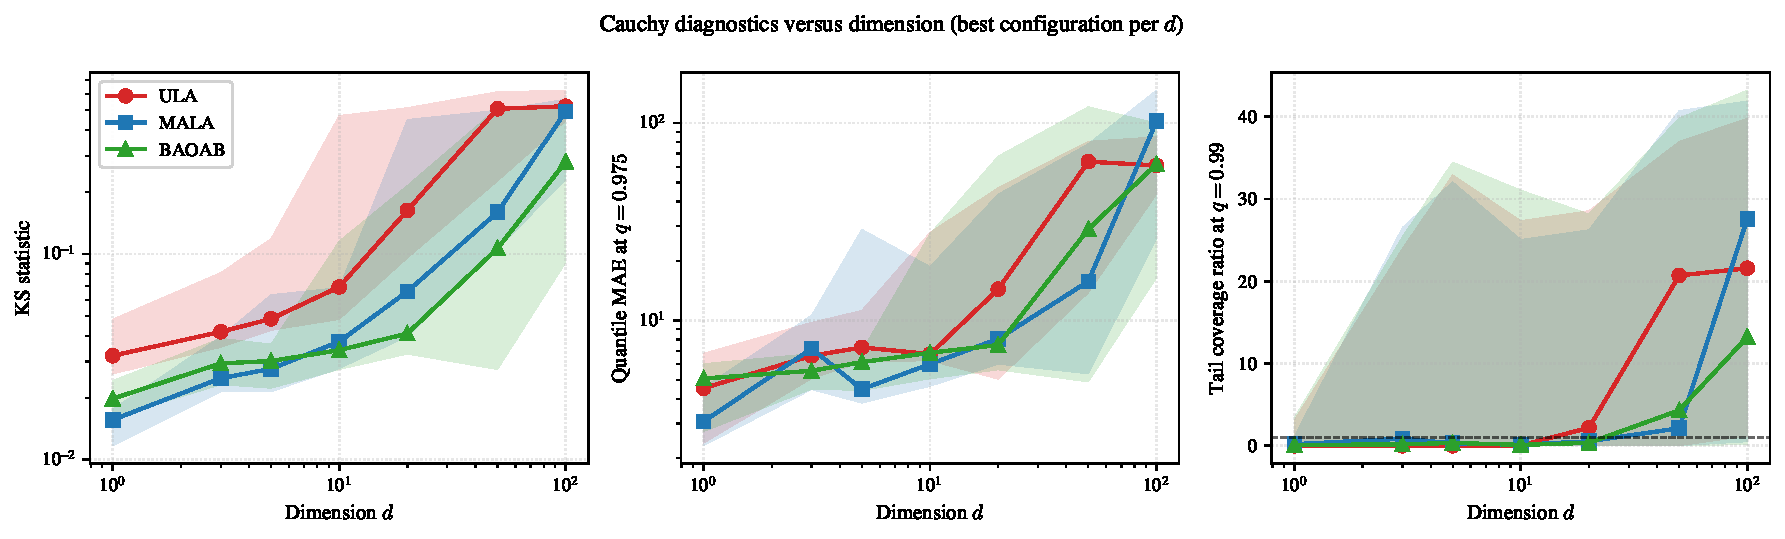
\includegraphics[width=\textwidth]{../../experiments/figures/original_thesis/cauchy_dimension_scaling}
\caption{Διαγνωστικά Cauchy ως συνάρτηση της διάστασης, στη βέλτιστη διαμόρφωση
ανά αλγόριθμο σε κάθε $d$. Αριστερά: διάμεση στατιστική KS. Μέσο: διάμεσο
q-MAE στο $q=0.975$. Δεξιά: διάμεση αναλογία κάλυψης ουράς στο $q=0.99$.
Οι σκιασμένες ζώνες αντιστοιχούν στο IQR μεταξύ $20$ εκτελέσεων. Η οριζόντια
διακεκομμένη γραμμή στο δεξί πλαίσιο σηματοδοτεί την ιδανική τιμή κάλυψης
ουράς $1.0$. Και τα τρία διαγνωστικά υποδηλώνουν αλλαγή καθεστώτος μεταξύ
$d=10$ και $d=50$, πέραν της οποίας η δειγματοληψία Cauchy γίνεται ουσιαστικά
μη εφαρμόσιμη σε $5\!\times\!10^4$ επαναλήψεις.}
\label{fig:cauchy-dim}
\end{figure}

Τρεις παρατηρήσεις ξεχωρίζουν:

\begin{itemize}
\item Και οι τρεις αλγόριθμοι υποβαθμίζονται ομαλά με τη διάσταση έως
      $d \approx 10$ και στη συνέχεια καταρρέουν ταχέως μεταξύ $d = 10$ και
      $d = 50$. Οι μέσες τιμές KS για τη βέλτιστη διαμόρφωση είναι:
      MALA $0.07 \to 0.16 \to 0.49$ για $d \in \{20, 50, 100\}$.
      BAOAB $0.04 \to 0.11 \to 0.28$. ULA $0.16 \to 0.51 \to 0.52$. Στο
      $d = 100$ και οι τρεις αλγόριθμοι αποτυγχάνουν λειτουργικά για την Cauchy
      στα εξεταζόμενα μήκη αλυσίδας --- όχι λόγω μηχανισμού ειδικού για κάποιον
      αλγόριθμο αλλά επειδή το τυπικό σύνολο μιας κατανομής βαριάς ουράς στο
      $\mathbb{R}^{100}$ είναι γεωμετρικά πολύ πιο δύσκολο να φτάσει από εκείνο
      του $\mathbb{R}^{1}$.
\item Ο BAOAB διατηρεί ένα περιθώριο έναντι του MALA στο q-MAE ποσοστημορίου
      Cauchy για μέτρια διάσταση (αριστερό πλαίσιο, καμπύλη BAOAB κάτω από
      εκείνη του MALA στο $d = 20$ και $d = 50$), αλλά στο $d = 100$ οι τρεις
      είναι ουσιαστικά ισόπαλοι στο ίδιο χαμηλό επίπεδο. Το πλεονέκτημα
      οδηγούμενο από ορμή του BAOAB που τεκμηριώνεται στην
      §\ref{sec:tail-correlation} εξασθενεί καθώς αυξάνεται το $d$.
\item Η κατανομή-στόχος Student-$t$ είναι πολύ πιο εύκολη από την Cauchy σε
      υψηλή διάσταση (Πίνακας~\ref{tab:dim-scaling-numbers}): η KS Student-$t$
      του BAOAB αυξάνεται μόνο από $0.008$ στο $d=1$ σε $0.013$ στο $d=100$.
      Αυτή η αντίθεση --- οι μέτριες ουρές είναι διαχειρίσιμες σε υψηλό $d$,
      οι ουρές χωρίς ροπές δεν είναι --- υποστηρίζει τη διατύπωση ολόκληρης
      της μελέτης με βάση τη βαρύτητα ουράς.
\end{itemize}

Η μελέτη περίπτωσης MALA στο $d=50$ στην Ενότητα~\ref{sec:case-mala-cauchy-d50}
δείχνει με αριθμούς αυτή την εικόνα για μία συγκεκριμένη διαμόρφωση.


\section{Μελέτες Περίπτωσης}
\label{sec:case-studies}

Για τη συμπλήρωση των συγκεντρωτικών μετρικών, επιλέγονται πέντε αντιπροσωπευτικές διαμορφώσεις και παρουσιάζονται τα τυπικά διαγνωστικά γραφήματα MCMC για μία 
  αλυσίδα: το \emph{trace plot} (η τιμή της πρώτης συντεταγμένης ανά επανάληψη), η \emph{συνάρτηση αυτοσυσχέτισης} (ACF, που μετρά τη συσχέτιση των δειγμάτων με  
  δείγματα $k$ βημάτων πριν) και ένα \emph{διάγραμμα καλής προσαρμογής} που συνδυάζει το εμπειρικό ιστόγραμμα με τα θεωρητικά ποσοστημόρια και ένα Q-Q plot       
  (εμπειρικά έναντι αναλυτικών ποσοστημορίων, με την τέλεια αντιστοίχιση να βρίσκεται στη διαγώνιο). Κάθε περίπτωση βασίζεται σε συγκεκριμένη εκτέλεση με το ίδιο 
  μήκος αλυσίδας που χρησιμοποιήθηκε στη μελέτη πλέγματος ($N=50{,}000$, burn-in $5{,}000$).

\begin{table}[H]
\centering
\small
\begin{tabular}{cllrrr}
\toprule
\# & Αλγόριθμος & Κατανομή-στόχος & $d$ & $\eta$ & $\gamma$ \\
\midrule
1 & MALA  & Γκαουσιανή      & $1$   & $1.0$ & --- \\
2 & ULA   & Γκαουσιανή      & $1$   & $0.30$ & --- \\
3 & ULA   & Cauchy        & $1$   & $0.10$ & --- \\
4 & BAOAB & Cauchy        & $1$   & $0.5$  & $0.5$ \\
5 & MALA  & Cauchy        & $50$  & $1.0$  & --- \\
\bottomrule
\end{tabular}
\caption{Οι πέντε διαμορφώσεις μελέτης περίπτωσης. Η Περίπτωση 1 δείχνει πώς
φαίνεται μια υγιής αλυσίδα. Οι Περιπτώσεις 2 και 3 δείχνουν δύο διακριτούς
τρόπους αποτυχίας του ULA (ήπια μεροληψία σε ελαφριές ουρές έναντι κατάρρευσης
ουράς σε βαριές ουρές). Η Περίπτωση 4 δείχνει πώς χειρίζεται μια καλά ρυθμισμένη
αλυσίδα BAOAB μια κατανομή-στόχο βαριάς ουράς στο $d=1$. Η Περίπτωση 5 δείχνει
πώς η ίδια κατανομή-στόχος γίνεται ποιοτικά δυσκολότερη για τον MALA στο
$d=50$.}
\label{tab:cases}
\end{table}

\subsection{Μελέτη Περίπτωσης 1 --- MALA Γκαουσιανή (αναφορά: υγιής αλυσίδα)}
\label{sec:case-mala-gauss}

Αυτή είναι η βέλτιστη διαμόρφωση MALA για τη Γκαουσιανή από τον
Πίνακα~\ref{tab:best-configs}: διάμεσος KS $0.0056$, αποδοχή $0.78$,
ESS $\approx 36{,}000$.

\begin{figure}[H]
\centering
\begin{subfigure}{\textwidth}
  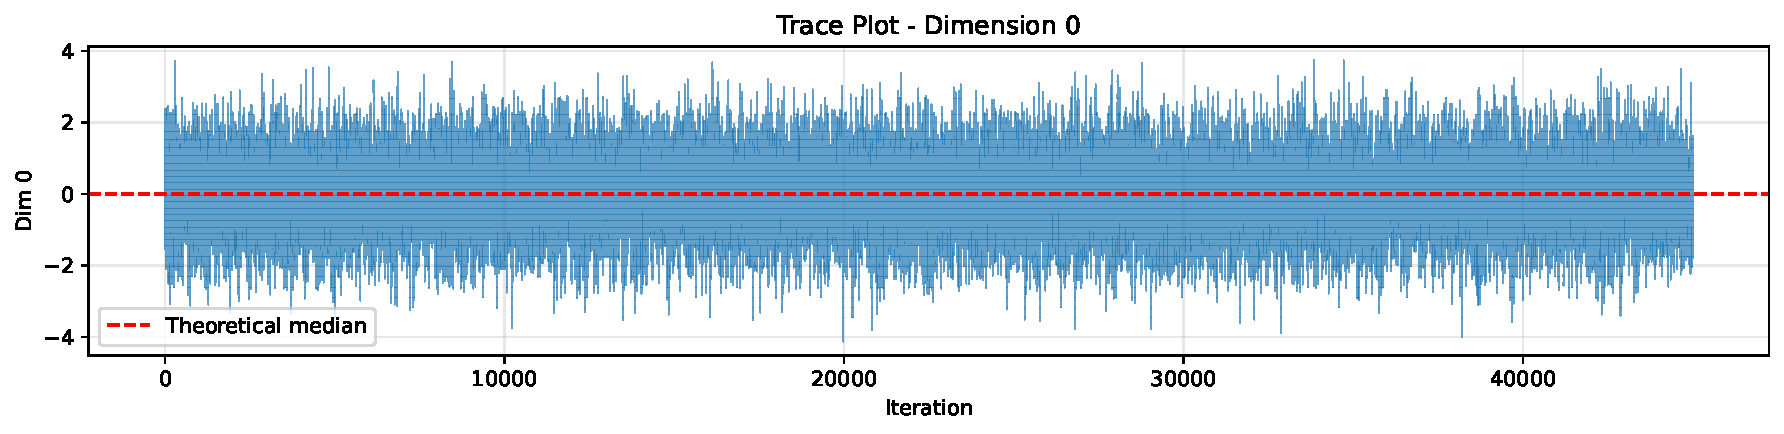
\includegraphics[width=\textwidth]{../../experiments/figures/original_thesis/case_studies/01_mala_gaussian_gold_standard_trace}
  \caption{Trace plot.}
\end{subfigure}\\[1ex]
\begin{subfigure}{0.42\textwidth}
  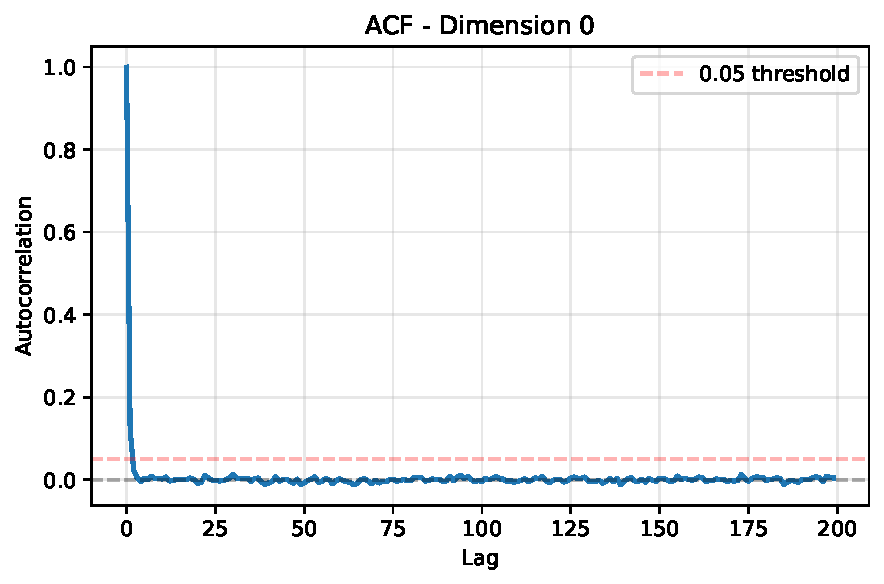
\includegraphics[width=\textwidth]{../../experiments/figures/original_thesis/case_studies/01_mala_gaussian_gold_standard_acf}
  \caption{Αυτοσυσχέτιση.}
\end{subfigure}\hfill
\begin{subfigure}{0.55\textwidth}
  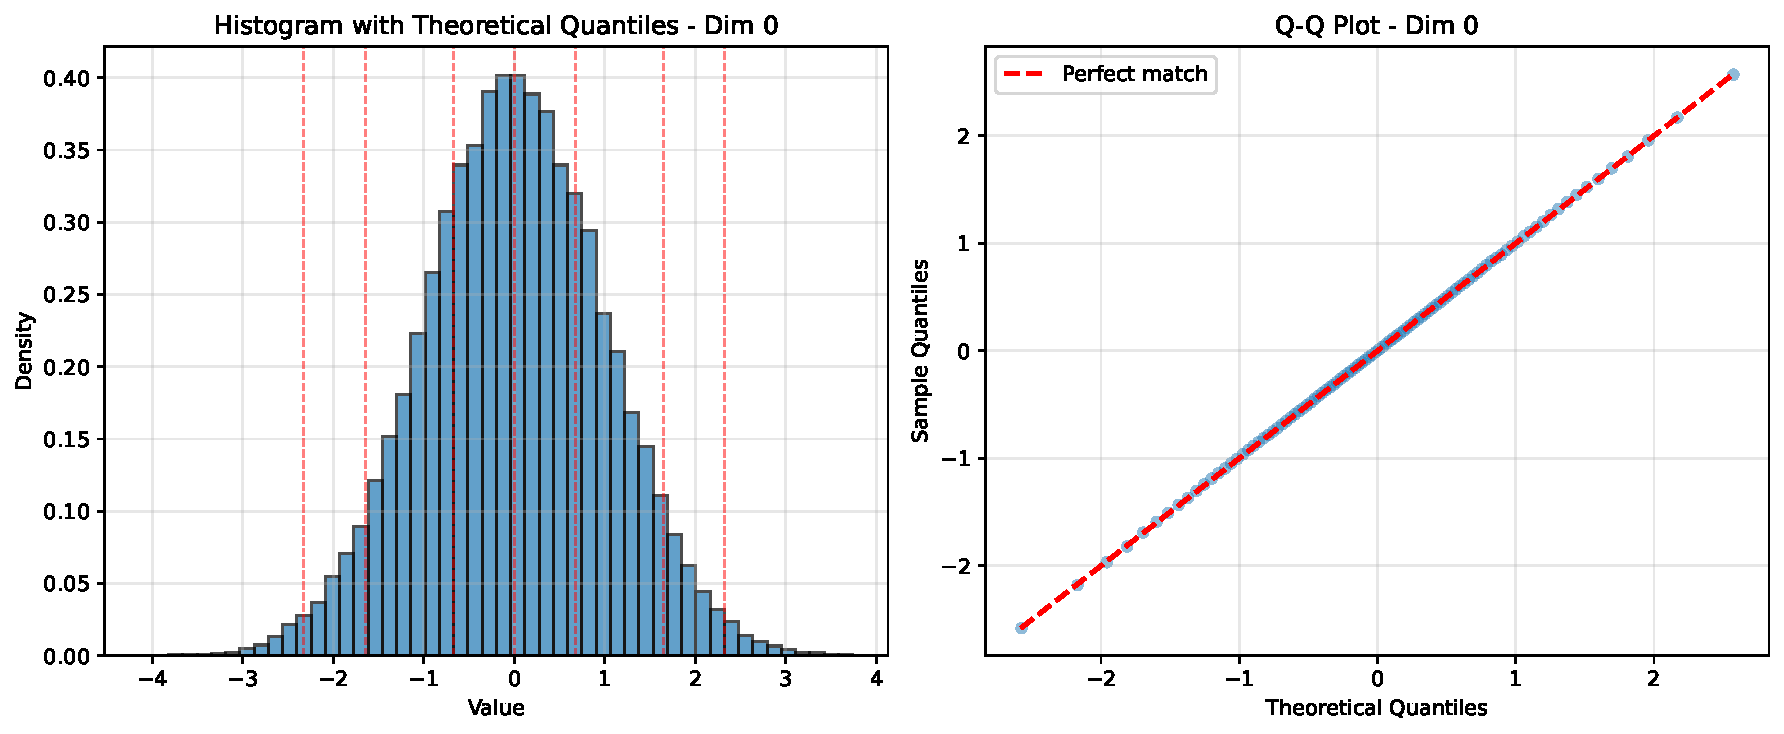
\includegraphics[width=\textwidth]{../../experiments/figures/original_thesis/case_studies/01_mala_gaussian_gold_standard_gof}
  \caption{Ιστόγραμμα με θεωρητικά ποσοστημόρια (αριστερά) και Q-Q plot (δεξιά).}
\end{subfigure}
\caption{Μελέτη Περίπτωσης 1: MALA στη Γκαουσιανή κατανομή-στόχο. Συμπεριφορά αναφοράς για σύγκριση με τις υπόλοιπες περιπτώσεις.}
\label{fig:case-mala-gauss}
\end{figure}

 Το trace plot κινείται ελεύθερα γύρω από το μηδέν χωρίς τάση ή
  αργή εκκίνηση. Η αυτοσυσχέτιση πέφτει κάτω από $0.05$ σε λίγα
  μόνο βήματα, πράγμα που σημαίνει ότι διαδοχικά δείγματα είναι
  σχεδόν ανεξάρτητα --- εξ ου και το υψηλό ESS $\approx 36{,}000$.
  Το Q-Q plot ακολουθεί τη διαγώνιο σε όλο το εύρος, και το
  ιστόγραμμα εφαρμόζει καλά στη θεωρητική Γκαουσιανή πυκνότητα.
  Οι υπόλοιπες μελέτες περίπτωσης θα πρέπει να διαβάζονται ως
  αποκλίσεις από αυτή την εικόνα.


\subsection{Μελέτη Περίπτωσης 2 --- ULA Γκαουσιανή (ήπιo bias διακριτοποίησης)}
\label{sec:case-ula-gauss}

\begin{figure}[H]
\centering
\begin{subfigure}{\textwidth}
  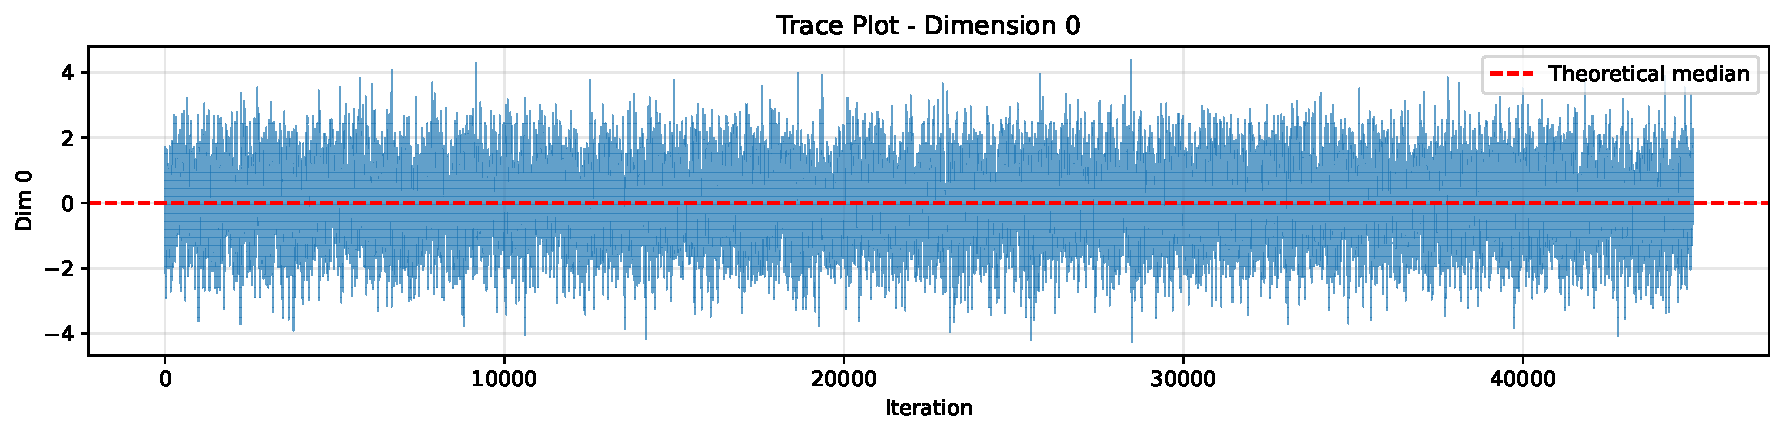
\includegraphics[width=\textwidth]{../../experiments/figures/original_thesis/case_studies/02_ula_gaussian_mild_bias_trace}
  \caption{Trace plot.}
\end{subfigure}\\[1ex]
\begin{subfigure}{0.42\textwidth}
  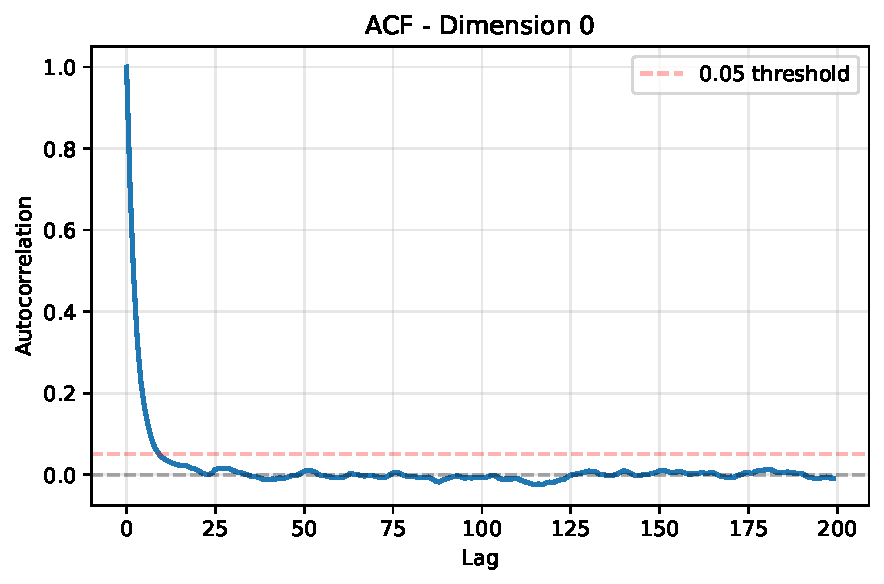
\includegraphics[width=\textwidth]{../../experiments/figures/original_thesis/case_studies/02_ula_gaussian_mild_bias_acf}
  \caption{Αυτοσυσχέτιση.}
\end{subfigure}\hfill
\begin{subfigure}{0.55\textwidth}
  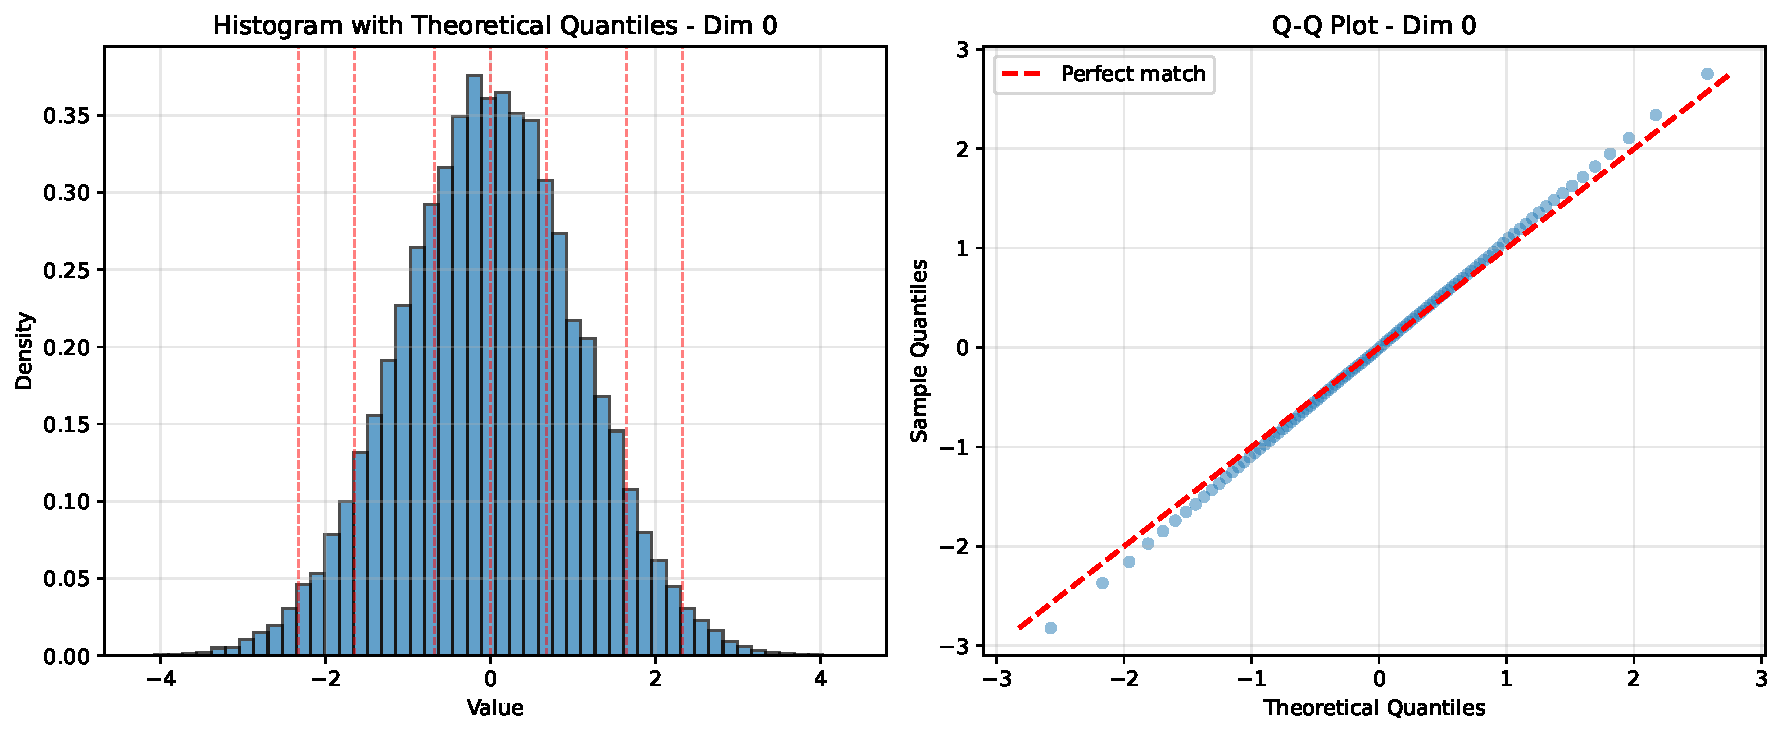
\includegraphics[width=\textwidth]{../../experiments/figures/original_thesis/case_studies/02_ula_gaussian_mild_bias_gof}
  \caption{Ιστόγραμμα και Q-Q plot.}
\end{subfigure}
\caption{Μελέτη Περίπτωσης 2: ULA στη Γκαουσιανή κατανομή-στόχο σε $\eta=0.30$.
Η αλυσίδα αναμειγνύεται καλά (το trace plot και η ACF φαίνονται κανονικά) αλλά
η στάσιμη κατανομή είναι ελαφρώς πλατύτερη από την κατανομή-στόχο.}
\label{fig:case-ula-gauss}
\end{figure}

Εξωτερικά αυτή η περίπτωση φαίνεται πανομοιότυπη με την Περίπτωση 1: το trace
plot είναι αυτό μιας υγιούς αλυσίδας και η ACF πέφτει καθαρά στο μηδέν έως
για lag $\sim 7$. Η μεροληψία εμφανίζεται μόνο στο πλαίσιο καλής προσαρμογής.
Το εμπειρικό ιστόγραμμα εκτείνεται ορατά πέραν των δεικτών θεωρητικού
ποσοστημορίου $97.5\%$ (στο $\pm 1.96$). Το Q-Q plot κάμπτεται ελαφρώς προς τα
έξω στα άκρα, υποδηλώνοντας ότι το εμπειρικό ποσοστημόριο $97.5\%$ της
αλυσίδας είναι ελαφρώς πιο ακραίο από το αναλυτικό. Η αλυσίδα αναμειγνύεται
αποδοτικά --- προς μια στάσιμη κατανομή ελαφρώς πλατύτερη από την
κατανομή-στόχο. Αυτό αποτελεί το χαρακτηριστικό αποτύπωμα της στατικής μεροληψίας
$\mathcal{O}(\eta)$ του ULA: μια αλυσίδα που φαίνεται υγιής βάσει διαγνωστικών
ανάμειξης αλλά της οποίας τα διαγνωστικά αντιστοίχισης κατανομής αποκαλύπτουν
το σφάλμα.

\subsection{Μελέτη Περίπτωσης 3 --- ULA Cauchy (κατάρρευση βαριάς ουράς)}
\label{sec:case-ula-cauchy}

\begin{figure}[H]
\centering
\begin{subfigure}{\textwidth}
  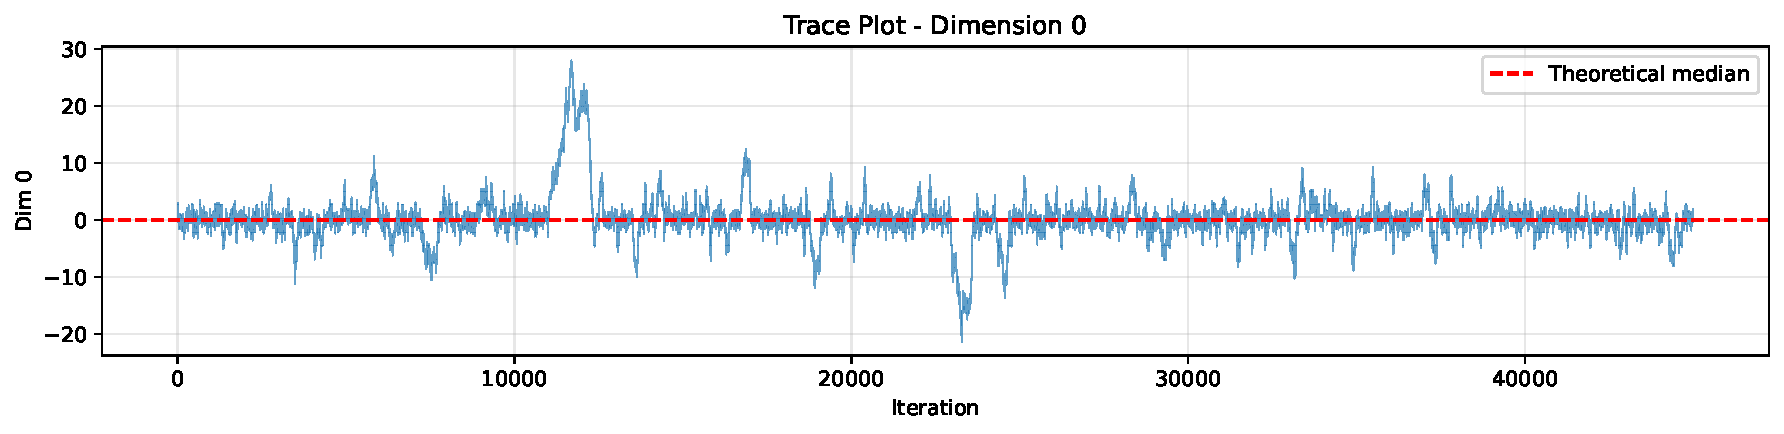
\includegraphics[width=\textwidth]{../../experiments/figures/original_thesis/case_studies/03_ula_cauchy_tail_collapse_trace}
  \caption{Trace plot.}
\end{subfigure}\\[1ex]
\begin{subfigure}{0.42\textwidth}
  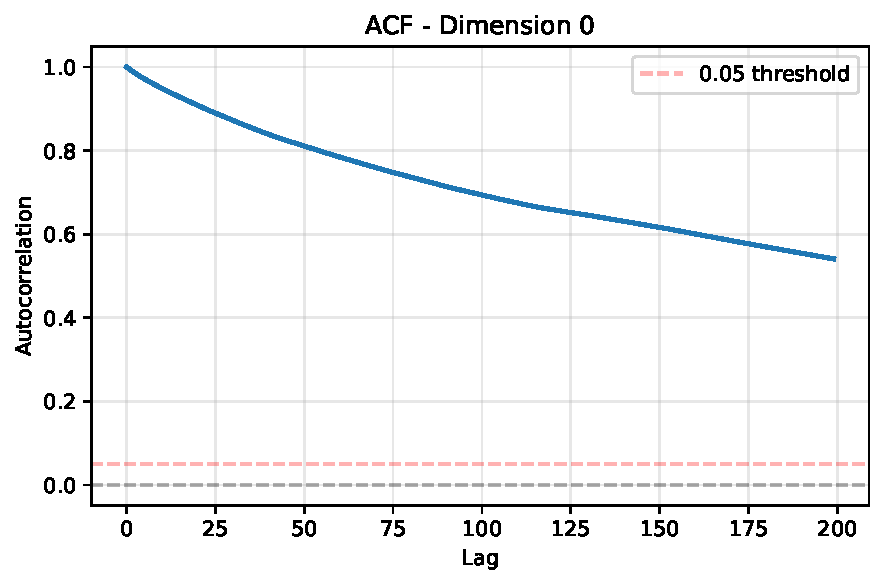
\includegraphics[width=\textwidth]{../../experiments/figures/original_thesis/case_studies/03_ula_cauchy_tail_collapse_acf}
  \caption{Αυτοσυσχέτιση.}
\end{subfigure}\hfill
\begin{subfigure}{0.55\textwidth}
  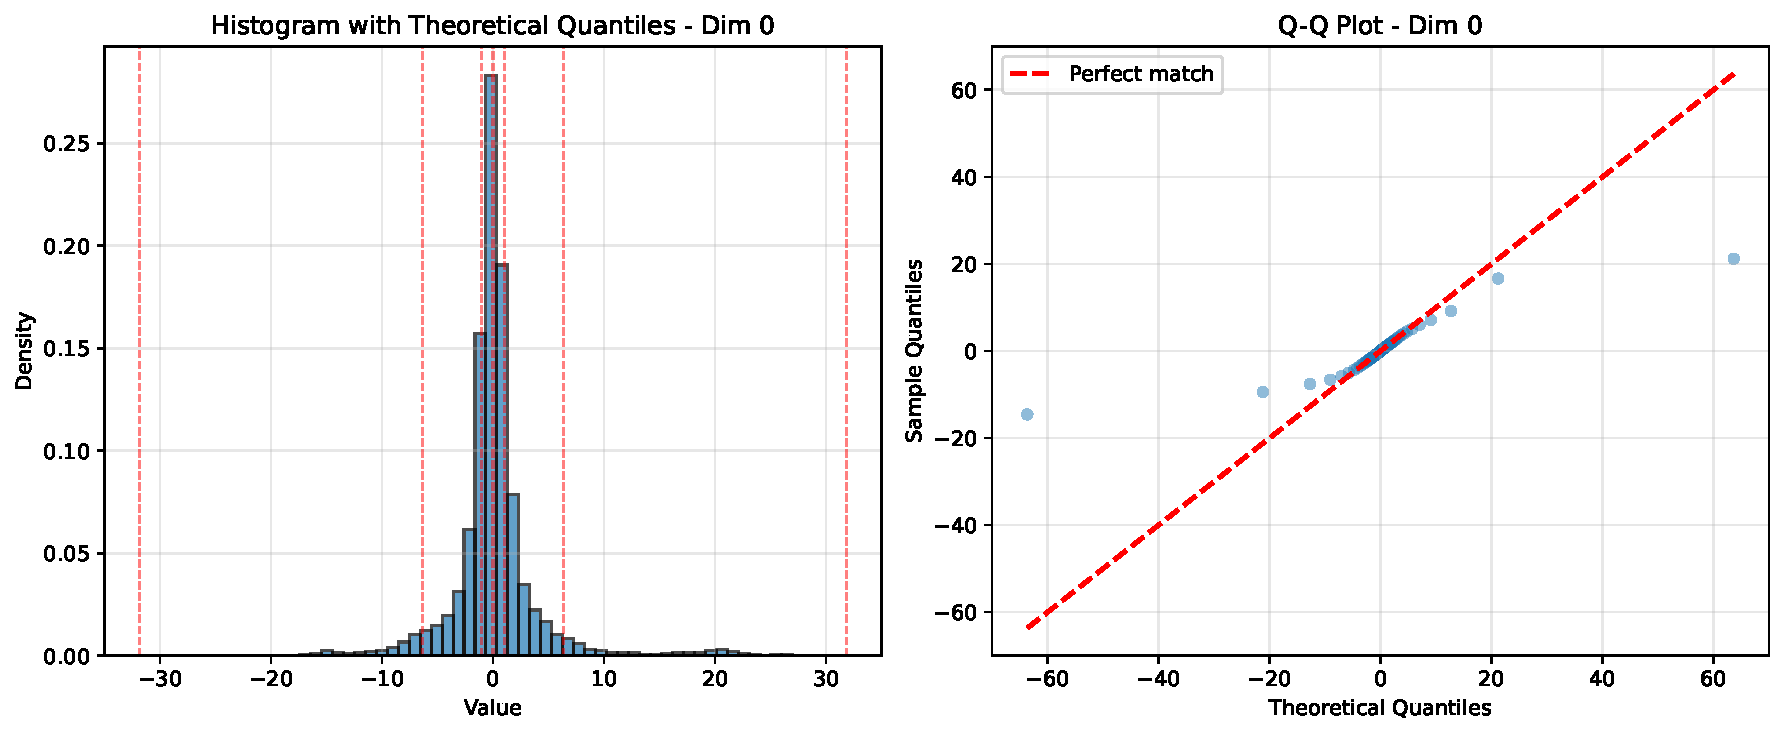
\includegraphics[width=\textwidth]{../../experiments/figures/original_thesis/case_studies/03_ula_cauchy_tail_collapse_gof}
  \caption{Ιστόγραμμα και Q-Q plot. Οι κατακόρυφες κόκκινες γραμμές σηματοδοτούν
  τα θεωρητικά ποσοστημόρια $1\%$ και $99\%$ της Cauchy στο $\pm 31.8$.}
\end{subfigure}
\caption{Μελέτη Περίπτωσης 3: ULA στην Cauchy κατανομή-στόχο σε $\eta=0.10$.
Η αλυσίδα φτάνει στο $|x|\approx 20$ σε περιστασιακές εκδρομές αλλά δεν μπορεί
να φτάσει σε μεγαλύτερες τιμές τα θεωρητικά ποσοστημόρια $1\%/99\%$ της Cauchy είναι στο
$\pm 31.8$.}
\label{fig:case-ula-cauchy}
\end{figure}

Αυτή είναι η κεντρική αποτυχία που τεκμηριώνεται στην εργασία. Το trace
plot δείχνει απομονωμένες εκδρομές από την αρχή που φτάνουν στο $|x| \approx 20$,
αλλά τα θεωρητικά ποσοστημόρια $1\%$ και $99\%$ της Cauchy βρίσκονται στο
$\pm 31.8$ --- η αλυσίδα απλώς δεν φτάνει εκεί σε $45{,}000$ δείγματα μετά το
burn-in. Το Q-Q plot φανερώνει το πρόβλημα καθαρά: τα πιο ακραία εμπειρικά
ποσοστημόρια στην αλυσίδα είναι πολύ μικρότερα (σε απόλυτη τιμή) από τα
αντίστοιχα θεωρητικά ποσοστημόρια. Η συνάρτηση αυτοσυσχέτισης καθιστά ρητή
την παθολογία ανάμειξης: σε υστέρηση $200$ η αυτοσυσχέτιση παραμένει γύρω στο
$0.5$, πολύ πάνω από το κατώφλι $0.05$ --- η αλυσίδα εξερευνά αργά ακόμη και
εντός της περιοχής που φτάνει.

Ο μηχανισμός είναι εκείνος που περιγράφεται στην Ενότητα~\ref{sec:tail-correlation}:
για το δυναμικό Cauchy, η ντετερμινιστική ολίσθηση της πρότασης ULA
$-\eta \nabla U(x)$ τείνει στο μηδέν καθώς $\|x\|\to\infty$, οπότε η αλυσίδα
δεν έχει τρόπο να μεροληπτεί είτε \emph{προς} είτε \emph{μακριά από} τις βαθιές
ουρές. Με θόρυβο πρότασης τάξης $\sqrt{2\eta} \approx 0.45$, η αναμενόμενη
μετατόπιση ανά βήμα είναι πολύ μικρότερη από την έκταση που καλύπτουν οι ουρές της κατανομής.

\subsection{Μελέτη Περίπτωσης 4 --- BAOAB Cauchy (καλύτερη διαχείριση βαριάς ουράς)}
\label{sec:case-baoab-cauchy}

\begin{figure}[H]
\centering
\begin{subfigure}{\textwidth}
  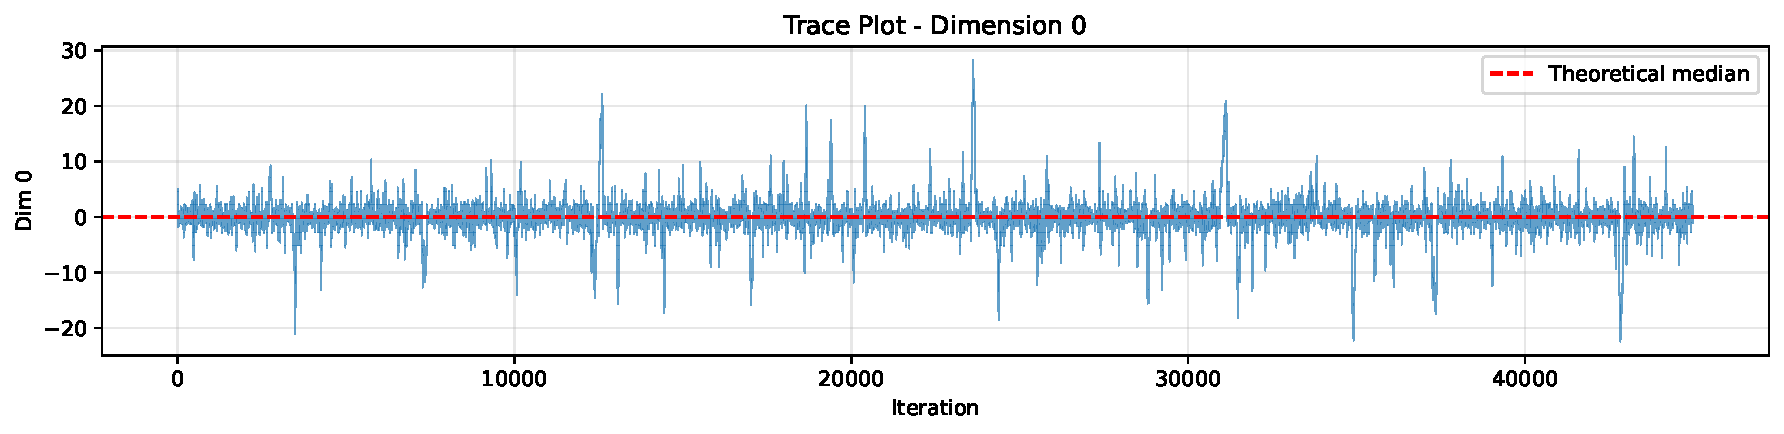
\includegraphics[width=\textwidth]{../../experiments/figures/original_thesis/case_studies/04_baoab_cauchy_best_trace}
  \caption{Trace plot. Σημειώστε τις μεγαλύτερες εκδρομές σε σύγκριση με την Περίπτωση 3.}
\end{subfigure}\\[1ex]
\begin{subfigure}{0.42\textwidth}
  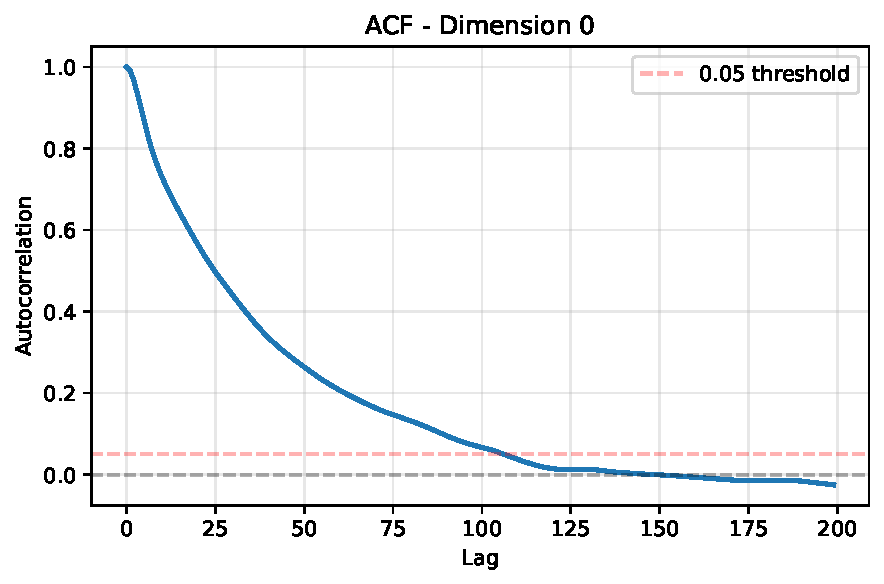
\includegraphics[width=\textwidth]{../../experiments/figures/original_thesis/case_studies/04_baoab_cauchy_best_acf}
  \caption{Αυτοσυσχέτιση.}
\end{subfigure}\hfill
\begin{subfigure}{0.55\textwidth}
  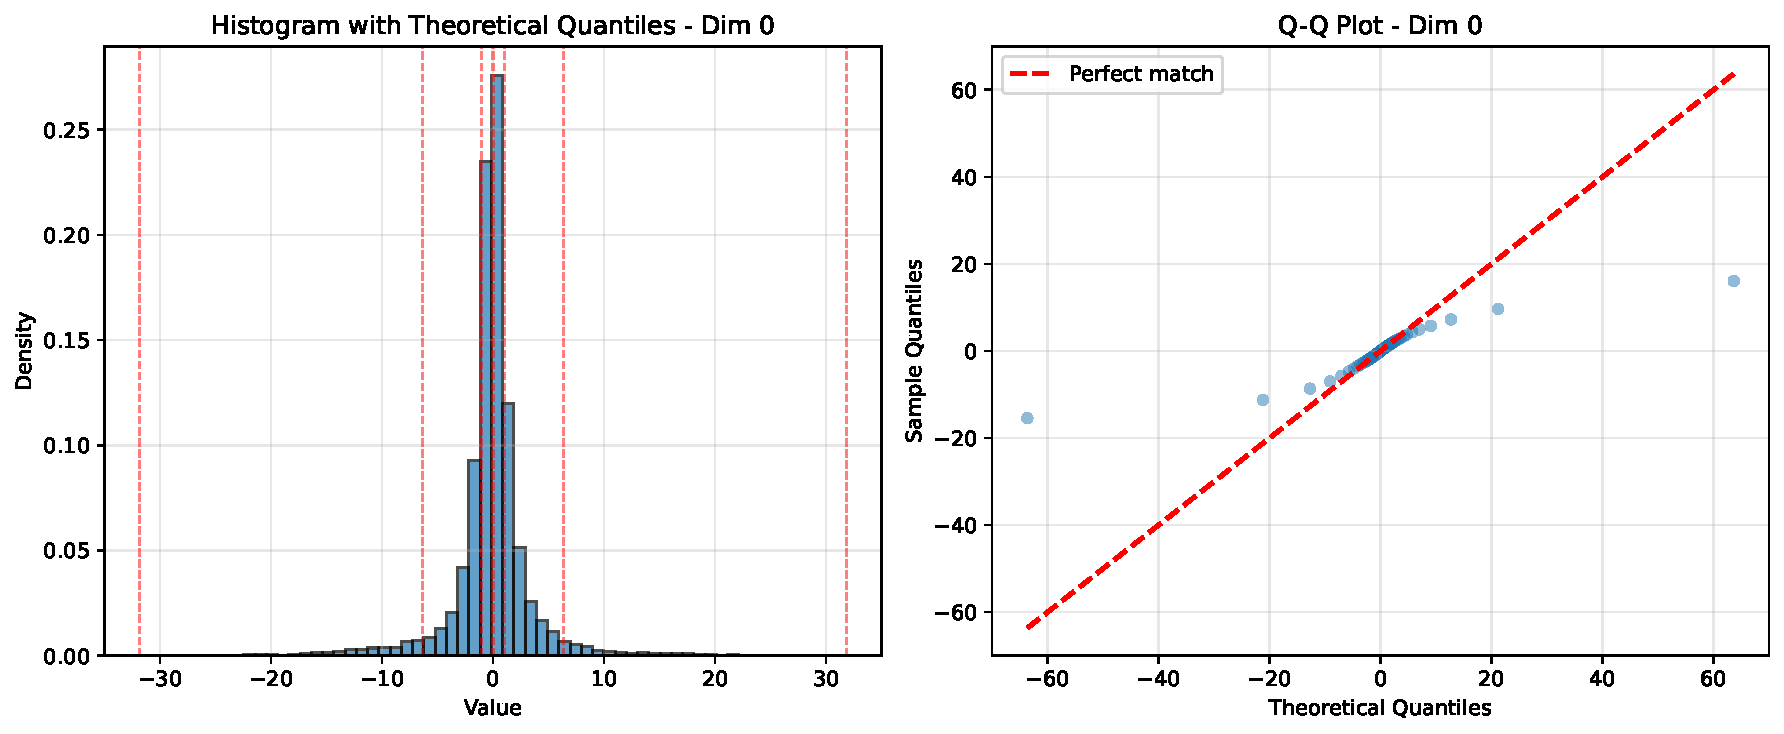
\includegraphics[width=\textwidth]{../../experiments/figures/original_thesis/case_studies/04_baoab_cauchy_best_gof}
  \caption{Ιστόγραμμα και Q-Q plot.}
\end{subfigure}
\caption{Μελέτη Περίπτωσης 4: BAOAB στην Cauchy κατανομή-στόχο σε $\eta=0.5$,
$\gamma=0.5$. Το trace plot δείχνει εκδρομές στο $\pm 28$ --- κοντά στα θεωρητικά
ποσοστημόρια $1\%/99\%$ στο $\pm 31.8$ --- τα οποία ο ULA στην Περίπτωση 3 δεν
μπορούσε να επιτύχει.}
\label{fig:case-baoab-cauchy}
\end{figure}

Σε σύγκριση με την Περίπτωση 3 για την ίδια κατανομή-στόχο, το trace plot του
BAOAB δείχνει ορατά μεγαλύτερες εκδρομές, που φτάνουν στο $|x| \approx 28$. Το
Q-Q plot είναι αντίστοιχα πιο κοντά στη διαγώνιο, και το ιστόγραμμα έχει μάζα
πέραν του $|x|=20$ που ο ULA δεν είχε ουσιαστικά καθόλου. Τα βαθύτερα εμπειρικά
ποσοστημόρια εξακολουθούν να υπολείπονται των αναλυτικών ποσοστημορίων Cauchy
στο $|x|=63$ (το εμπειρικό ποσοστημόριο $0.5\%$), αλλά το χάσμα είναι πολύ
μικρότερο από εκείνο του ULA. Σε αυτό το μήκος αλυσίδας η ουρά εξερευνάται
μερικώς. Η μελέτη σύγκλισης στην Ενότητα~\ref{sec:convergence-study} δείχνει
ότι με μεγαλύτερη αλυσίδα ο BAOAB συνεχίζει να βελτιώνεται στην κάλυψη ουράς.

Η εξήγηση για το πλεονέκτημα του BAOAB έναντι του ULA στην Cauchy
είναι η αναλυτική ενημέρωση Ornstein--Uhlenbeck στην ορμή,
$V \mapsto e^{-\gamma\eta} V + \sqrt{1 - e^{-2\gamma\eta}}\,\xi$, η οποία
εισάγει θόρυβο στη μεταβλητή ταχύτητας αντί απευθείας στη θέση. Η συσσωρευμένη
ορμή μπορεί να οδηγεί τη θέση σε πολλά βήματα μισής ολίσθησης πριν αποσβεστεί
από το επόμενο O-βήμα, επιτρέποντας στην αλυσίδα να διανύσει μεγάλες αποστάσεις
χωρίς να απαιτείται ένα ξαφνικό μεγάλο άλμα σε μία μόνο επανάληψη. Ο ULA δεν έχει
σύζευξη ορμής και επομένως δεν μπορεί να συσσωρεύσει μετατόπιση μεταξύ
επαναλήψεων με αυτόν τον τρόπο.

\subsection{Μελέτη Περίπτωσης 5 --- MALA Cauchy σε $d=50$ (βαριές ουρές σε μέτρια διάσταση)}
\label{sec:case-mala-cauchy-d50}

Αυτή η περίπτωση χρησιμοποιεί τον ίδιο αλγόριθμο με την Περίπτωση 1 (MALA)
για την ίδια κατανομή-στόχο με τις Περιπτώσεις 3--4 (Cauchy), αλλά σε διάσταση
$d=50$ αντί για $d=1$. Το βέλτιστο $\eta$ στο $d=50$ είναι $1.0$ (έναντι $4.0$
στο $d=1$, δείχνοντας την εμπειρική κλιμάκωση βήματος που συζητείται στην
Ενότητα~\ref{sec:dim-scaling}). Αναφερόμενες μετρικές από τον
Πίνακα~\ref{tab:cases}: διάμεσος KS $0.16$, αποδοχή $0.77$, ESS $\approx 108$.

\begin{figure}[H]
\centering
\begin{subfigure}{\textwidth}
  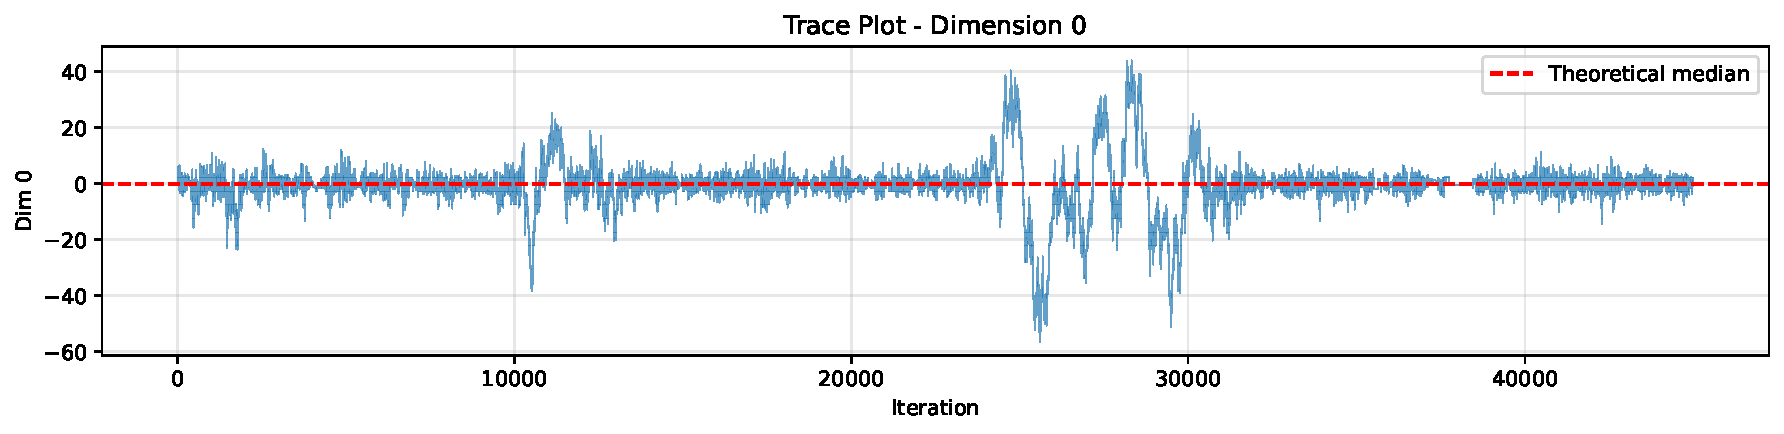
\includegraphics[width=\textwidth]{../../experiments/figures/original_thesis/case_studies/05_mala_cauchy_d50_trace}
  \caption{Trace plot.}
\end{subfigure}\\[1ex]
\begin{subfigure}{0.42\textwidth}
  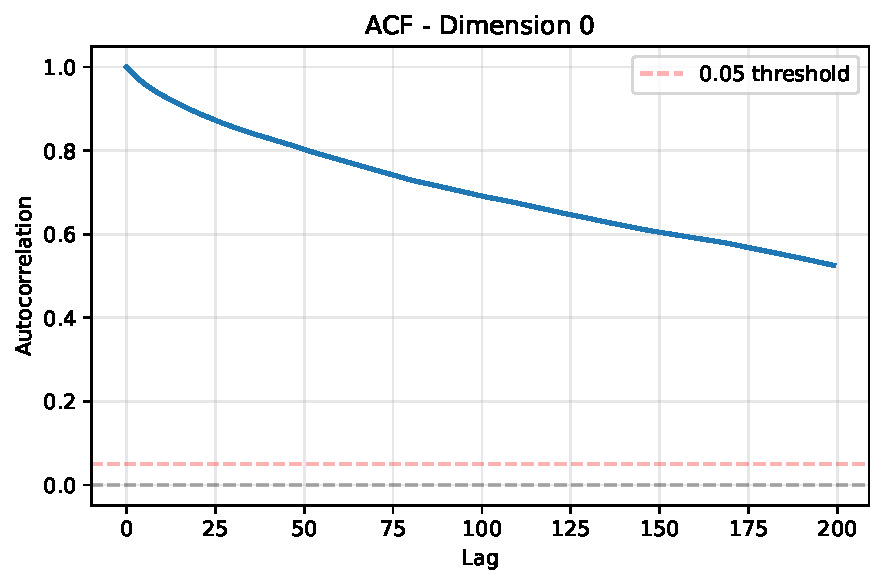
\includegraphics[width=\textwidth]{../../experiments/figures/original_thesis/case_studies/05_mala_cauchy_d50_acf}
  \caption{Αυτοσυσχέτιση.}
\end{subfigure}\hfill
\begin{subfigure}{0.55\textwidth}
  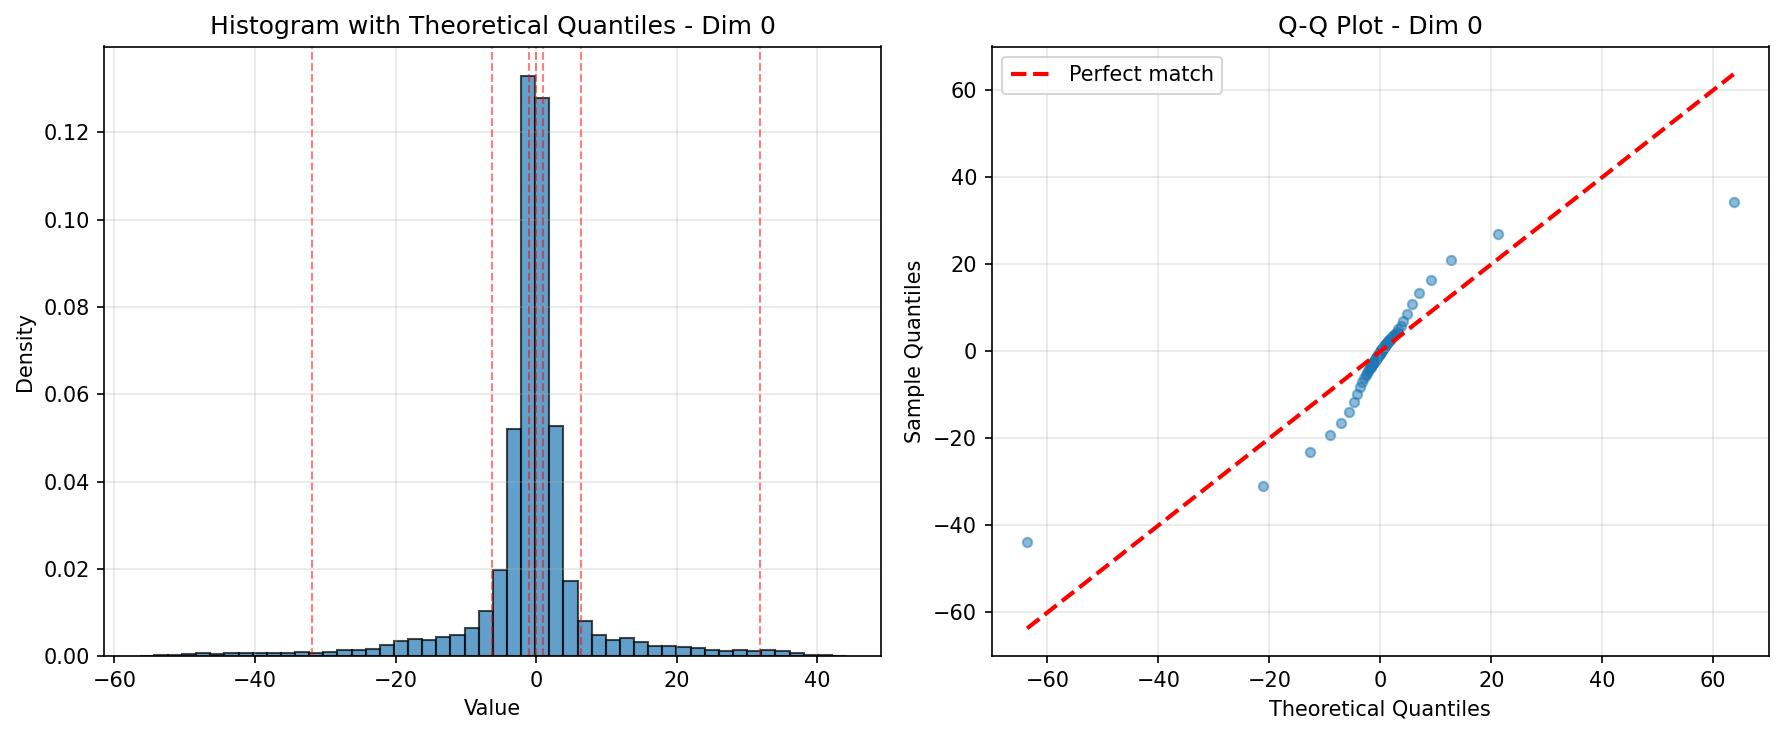
\includegraphics[width=\textwidth]{../../experiments/figures/original_thesis/case_studies/05_mala_cauchy_d50_gof}
  \caption{Ιστόγραμμα και Q-Q plot.}
\end{subfigure}
\caption{Μελέτη Περίπτωσης 5: MALA στην Cauchy κατανομή-στόχο σε $d=50$,
$\eta=1.0$. Η αλυσίδα φτάνει στο $|x| \approx 60$ σε περιστασιακές εκδρομές
αλλά περνά μακρά διαστήματα κοντά στην αρχή μεταξύ τους. Το ESS σε αυτή τη
διαμόρφωση είναι $\approx 108$ για $45{,}000$ δείγματα μετά το burn-in,
μείωση κατά τρεις τάξεις μεγέθους σε σύγκριση με τον MALA στη Γκαουσιανή κατανομή-στόχο για το ίδιο μήκος αλυσίδας.}
\label{fig:case-mala-cauchy-d50}
\end{figure}

Το trace plot δείχνει το ποιοτικό αποτύπωμα της δειγματοληψίας βαριάς ουράς
υψηλής διάστασης: μακρές ήσυχες περίοδοι κοντά στην αρχή που διακόπτονται από
σπάνιες εκρήξεις μεγάλων εκδρομών, με τις εκρήξεις να διαρκούν χιλιάδες
επαναλήψεις αντί για λίγα βήματα. Η συνάρτηση αυτοσυσχέτισης φθίνει πολύ πιο
αργά από οποιαδήποτε από τις άλλες μελέτες περίπτωσης, και το Q-Q plot δείχνει
μερική αλλά ελλιπή κάλυψη ουράς. Η αλυσίδα δεν έχει κολλήσει (αποδοχή $0.77$)
αλλά ο αποτελεσματικός χρόνος ανάμειξής της είναι δραματικά πιο αργός από ό,τι
στο $d=1$.

Η περίπτωση δείχνει το κεντρικό συμπέρασμα της
Ενότητας~\ref{sec:dim-dependence-tails}: η δειγματοληψία βαριάς ουράς σε μέτρια
διάσταση είναι ποιοτικά διαφορετική από τη δειγματοληψία βαριάς ουράς στο $d=1$.
Η στρατηγική προσαρμογής-μέσω-μεγαλύτερων-βημάτων του MALA συνεχίζει να
λειτουργεί αλλά με πολύ μειωμένη αποδοτικότητα δειγματοληψίας.

\subsection{Τι Δείχνουν οι Μελέτες Περίπτωσης}

Οι πέντε περιπτώσεις φανερώνουν τα ευρήματα των
προηγούμενων ενοτήτων. Η αντίθεση μεταξύ Περιπτώσεων 1 και 2 απομονώνει τη
μόνιμη μεροληψία του ULA σε ελαφριά κατανομή-στόχο: η αλυσίδα αναμειγνύεται καλά
αλλά στοχεύει σε μια ελαφρώς λανθασμένη κατανομή. Η αντίθεση μεταξύ Περιπτώσεων
2 και 3 απομονώνει την επίδραση της βαρύτητας ουράς στη συμπεριφορά του ULA: η
ίδια ήπια υπερ-κάλυψη στη Γκαουσιανή γίνεται πλήρης κατάρρευση ουράς στην
Cauchy, με την αυτοσυσχέτιση υστέρησης-100 να αυξάνεται από $\sim 0$ σε
$\sim 0.5$. Η αντίθεση μεταξύ Περιπτώσεων 3 και 4 απομονώνει τον ρόλο του
ολοκληρωτή: και οι δύο αλγόριθμοι είναι μεροληπτικοί (χωρίς έλεγχο Metropolis)
και στοχεύουν στην ίδια Cauchy, αλλά ο splitting ολοκληρωτής BAOAB επιτυγχάνει
ουσιαστικά καλύτερη εξερεύνηση ουράς από το απλό βήμα Euler του ULA. Τέλος, η
Περίπτωση 5 απομονώνει τον ρόλο της διάστασης: ο ίδιος αλγόριθμος (MALA) για
την ίδια κατανομή-στόχο (Cauchy) στο $d=50$ αντί για $d=1$ έχει την αποδοτικότητα
δειγματοληψίας του μειωμένη κατά τρεις τάξεις μεγέθους σε ESS.


\section{Μελέτη Σύγκλισης στις Βέλτιστες Διαμορφώσεις}
\label{sec:convergence-study}

\subsection{Σχεδιασμός}

Μια ξεχωριστή μελέτη αντιμετωπίζει το ερώτημα: καθώς αυξάνεται το μήκος
αλυσίδας, πώς εξελίσσονται τα διαγνωστικά; Εκτελούμε καθεμία από τις εννέα
βέλτιστες διαμορφώσεις (αλγόριθμος, κατανομή) από τον Πίνακα~\ref{tab:best-configs}
για $10^6$ επαναλήψεις και υπολογίζουμε τις μετρικές σε τέσσερα σημεία ελέγχου
$N \in \{5\!\cdot\!10^4, 10^5, 5\!\cdot\!10^5, 10^6\}$. Όπως στη μελέτη
πλέγματος, κάθε διαμόρφωση εκτελείται με $10$ ανεξάρτητες εκτελέσεις (η καθεμία
χρησιμοποιεί το ίδιο υπέρ-διεσπαρμένο σχήμα αρχικής κατάστασης που περιγράφεται
στην Ενότητα~\ref{sec:init-state}), και αναφέρουμε διάμεσο και IQR μεταξύ
εκτελέσεων σε κάθε σημείο ελέγχου. Το σημείο ελέγχου $5 \times 10^4$
αντιστοιχεί στο μήκος αλυσίδας της προηγούμενης μελέτης πλέγματος, οπότε το αριστερότερο σημείο κάθε καμπύλης σύγκλισης συμπίπτει με την αντίστοιχη γραμμή του
Πίνακα~\ref{tab:best-configs}. Το σημείο ελέγχου $10^6$ είναι είκοσι φορές
μεγαλύτερο. Για μια αλυσίδα που δειγματοληπτεί σωστά, το KS θα
έπρεπε να φθίνει κατά $1/\sqrt{N}$ μεταξύ σημείων ελέγχου --- που στην
περίπτωσή μας θα αντιστοιχούσε σε μείωση κατά παράγοντα $\sqrt{20} \approx 4.5$
μεταξύ $5\times 10^4$ και $10^6$ επαναλήψεων, ισοδύναμη με αναλογία $0.224$.

\subsection{Σύγκλιση KS}

\begin{figure}[ht]
\centering
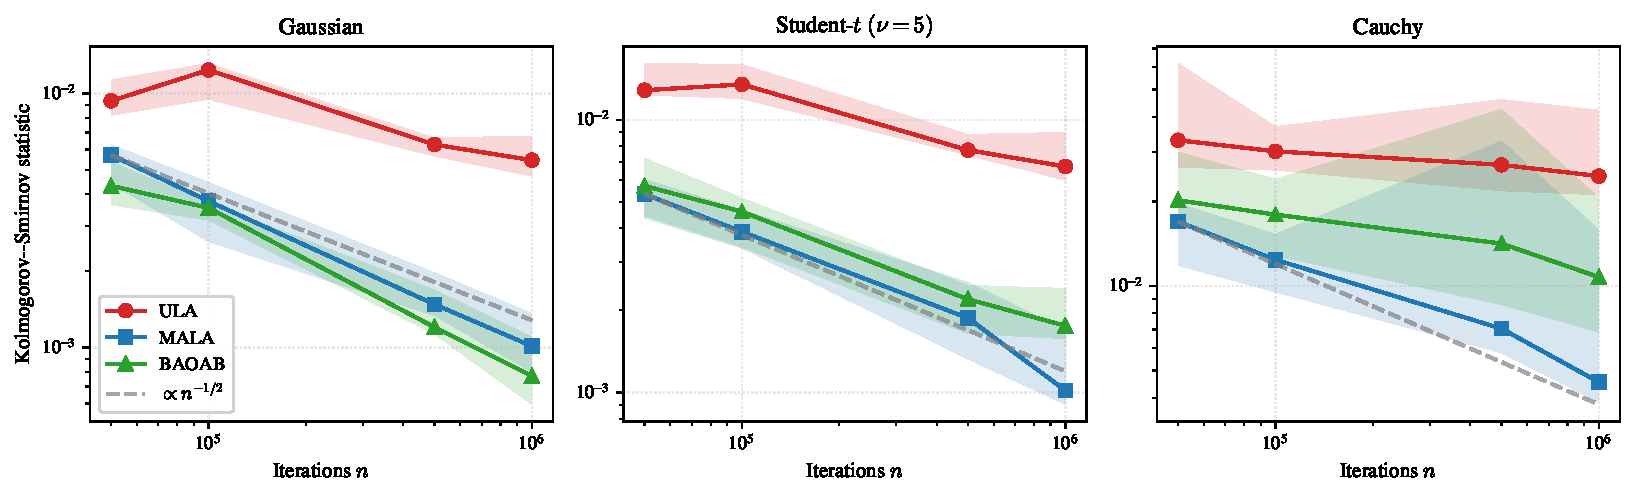
\includegraphics[width=\textwidth]{../../experiments/figures/original_thesis/ks_convergence}
\caption{Στατιστική Kolmogorov--Smirnov ως συνάρτηση του μήκους αλυσίδας, σε
λογαριθμική κλίμακα. Κάθε γραμμή είναι η διάμεση τιμή KS μεταξύ $10$ εκτελέσεων. Η
σκιασμένη ζώνη είναι το IQR. Η διακεκομμένη γκρι γραμμή είναι η κλίση αναφοράς
$N^{-1/2}$ που προβλέπεται από την κλασική θεωρία για αλυσίδα που στοχεύει
σωστά στην $\pi$.}
\label{fig:ks-conv}
\end{figure}

Ο Πίνακας~\ref{tab:ks-conv-ratio} συνοψίζει την αναλογία μείωσης μεταξύ ελάχιστου
και μέγιστου μήκους αλυσίδας. Υπενθυμίζουμε ότι $0.224$ είναι η ιδανική τιμή
$1/\sqrt{N}$.

\begin{table}[ht]
\centering
\small
\begin{tabular}{lccc}
\toprule
Αλγόριθμος & Γκαουσιανή & Student-$t$ & Cauchy \\
\midrule
ULA   & $0.58\times$ & $0.52\times$ & $0.75\times$ \\
MALA  & $\mathbf{0.18\times}$ & $\mathbf{0.19\times}$ & $\mathbf{0.27\times}$ \\
BAOAB & $\mathbf{0.18\times}$ & $0.31\times$ & $0.53\times$ \\
\bottomrule
\end{tabular}
\caption{Αναλογία μείωσης διαμέσου KS μεταξύ $N=5\times10^4$ και $N=10^6$.
Η κλασική πρόβλεψη $1/\sqrt{N}$ είναι $0.224\times$. Με έντονη γραφή
σηματοδοτούνται αναλογίες εντός παράγοντα δύο από την πρόβλεψη.}
\label{tab:ks-conv-ratio}
\end{table}

Η εικόνα είναι σαφής. Για τη Γκαουσιανή και τη Student-$t$ κατανομή-στόχο,
ο MALA και ο BAOAB επιτυγχάνουν αμφότεροι μειώσεις KS κοντά στον κλασικό ρυθμό
$1/\sqrt{N}$ --- δηλαδή η μετρική κυριαρχείται από τυχαίο σφάλμα Monte Carlo και
όχι από αλγοριθμική μεροληψία. Η KS του ULA πέφτει μεν, αλλά με πολύ πιο αργό
ρυθμό, υποδηλώνοντας ότι η μεροληψία του γίνεται η κυρίαρχη πηγή σφάλματος:
μακρύτερες αλυσίδες μειώνουν κατά μέσο όρο το τυχαίο σφάλμα αλλά δεν μπορούν
να αφαιρέσουν το κατώφλι μεροληψίας. Για την Cauchy, ο MALA συνεχίζει να
συγκλίνει κοντά στον ρυθμό $1/\sqrt{N}$, ο BAOAB σε περίπου τον μισό αυτόν τον
ρυθμό, και ο ULA μόλις κινείται πάνω από την εικοσαπλάσια αύξηση μεγέθους
δείγματος.

Οι απόλυτες τιμές KS στο $N = 10^6$ είναι: Γκαουσιανή --- BAOAB $0.0008$,
MALA $0.0010$, ULA $0.0055$. Student-$t$ --- MALA $0.0010$, BAOAB $0.0018$,
ULA $0.0067$. Cauchy --- MALA $0.0046$, BAOAB $0.0108$, ULA $0.0246$. Η Cauchy
είναι πραγματικά δύσκολη: στις $10^6$ επαναλήψεις ο MALA και ο BAOAB έχουν
τιμές KS κοντά στο σημείο που είχαν ο MALA και ο BAOAB στη Γκαουσιανή στις
$5\times 10^4$ επαναλήψεις.

\subsection{Κλιμάκωση ESS}

Το ESS θα πρέπει να αυξάνεται γραμμικά με το μήκος αλυσίδας εάν η αλυσίδα
βρίσκεται σε σταθερή-κατάσταση ανάμειξης. Το Σχήμα~\ref{fig:ess-scaling}
απεικονίζει το ESS ως συνάρτηση του $N$. Μια αλυσίδα που αναμειγνύεται με
σταθερό ρυθμό παράγει ευθεία γραμμή κλίσης ένα στους λογαριθμικούς άξονες.
Η διακεκομμένη γραμμή είναι η κλίση αναφοράς γραμμική-σε-$N$.

\begin{figure}[ht]
\centering
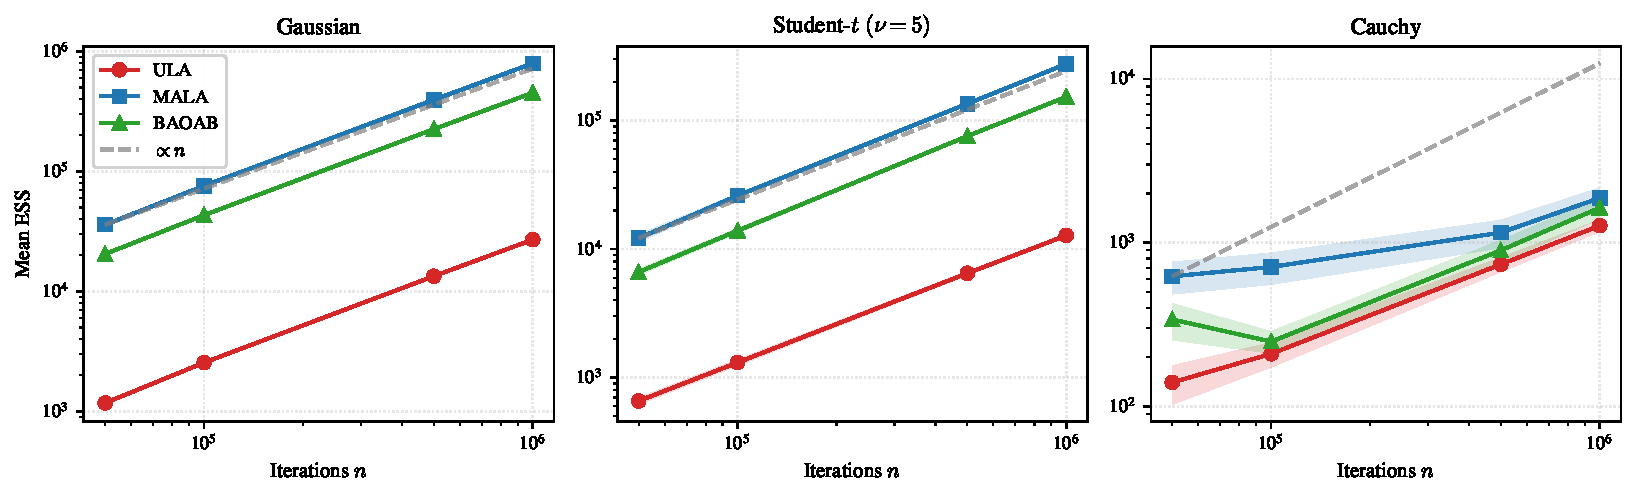
\includegraphics[width=\textwidth]{../../experiments/figures/original_thesis/ess_scaling}
\caption{Μέσο ESS ως συνάρτηση του μήκους αλυσίδας, διάμεση τιμή μεταξύ $10$
εκτελέσεων, με ζώνη $\pm$ τυπικό σφάλμα. Η διακεκομμένη γραμμή είναι η κλίση
αναφοράς γραμμική-σε-$N$.}
\label{fig:ess-scaling}
\end{figure}

Για τη Γκαουσιανή και τη Student-$t$, και οι τρεις αλγόριθμοι εκδηλώνουν
κλιμάκωση ESS κοντά στη γραμμική (αναλογία περίπου $20\times$ μεταξύ
$N=5\times 10^4$ και $N=10^6$). Για την Cauchy η κλιμάκωση είναι υπογραμμική:
μεταξύ των ίδιων δύο ακρών το ESS πολλαπλασιάζεται μόνο $3\times$ για τον MALA,
$5\times$ για τον BAOAB και $9\times$ για τον ULA. Η ερμηνεία είναι ότι
περιστασιακές μακρές εκδρομές στις ουρές της Cauchy κρατούν τον ολοκληρωμένο
χρόνο αυτοσυσχέτισης \emph{αυξανόμενο} με το μήκος αλυσίδας --- όσο μεγαλύτερη
η αλυσίδα, τόσο περισσότερες τέτοιες εκδρομές εμφανίζονται, και η καθεμία
διογκώνει τη συσχέτιση.

\subsection{Σύγκλιση q-MAE Ποσοστημορίου}

\begin{figure}[ht]
\centering
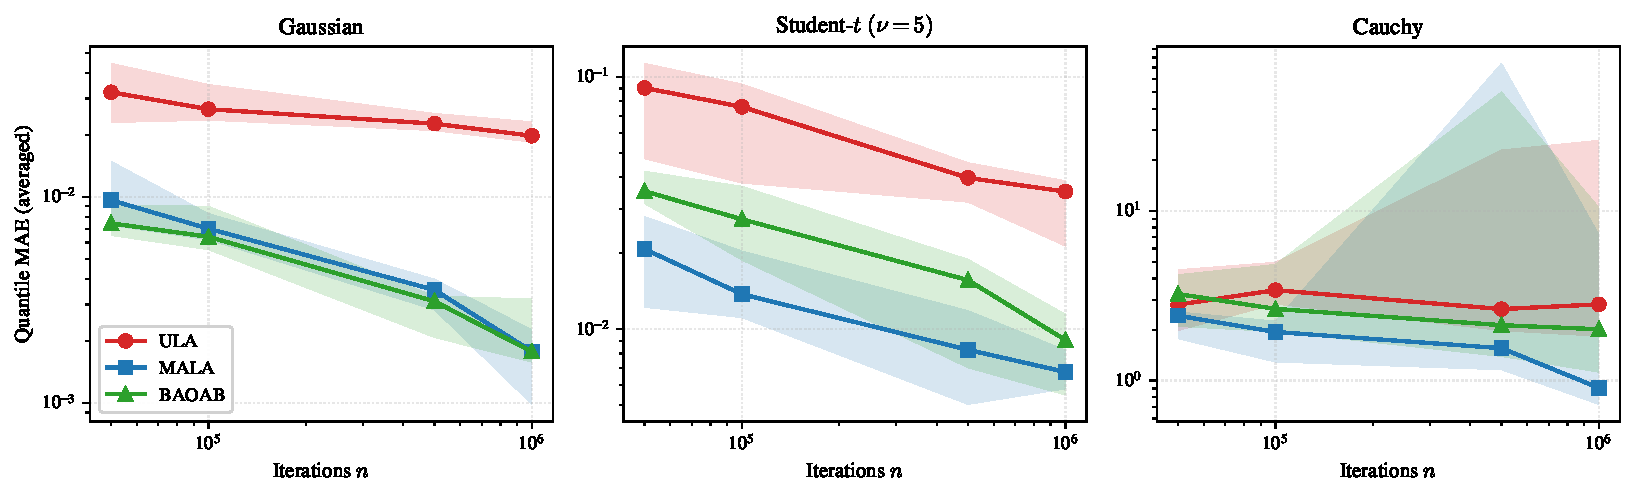
\includegraphics[width=\textwidth]{../../experiments/figures/original_thesis/quantile_mae_convergence}
\caption{Μέσο q-MAE ποσοστημορίου ως συνάρτηση του μήκους αλυσίδας, διάμεση τιμή
μεταξύ $10$ εκτελέσεων με ζώνη IQR.}
\label{fig:qmae-conv}
\end{figure}

Το q-MAE συμπεριφέρεται παρόμοια με το KS για τη Γκαουσιανή και τη Student-$t$:
ο MALA και ο BAOAB φθίνουν σταθερά, ο ULA ισοπεδώνεται. Για την Cauchy η εικόνα
είναι διαφορετική. Το q-MAE στις $10^6$ επαναλήψεις είναι $2.04$ για τον BAOAB,
$4.74$ για τον MALA και $4.81$ για τον ULA. \emph{Ο BAOAB έχει το καλύτερο q-MAE
για την Cauchy παρόλο που έχει υψηλότερο KS από τον MALA}: η στατιστική KS
κυριαρχείται από τον κορμό της κατανομής, αλλά το q-MAE στα άκρα κυριαρχείται
από το πόσο καλά φτάνει η αλυσίδα στις βαθιές ουρές. Ο BAOAB, χάρη στην ορμή του, καταγράφει καλύτερα τα ακραία ποσοστημόρια σε
σύγκριση με τον MALA, ο οποίος περιορίζεται από το ποσοστό αποδοχής. Η
επιλογή μεταξύ των δύο εξαρτάται από τις ανάγκες της εφαρμογής: αν
προτεραιότητα είναι η καλή προσαρμογή στον κορμό της κατανομής, ο MALA είναι
προτιμότερος για την Cauchy. Αν προτεραιότητα είναι η ακρίβεια στις ουρές,
ο BAOAB είναι προτιμότερος.

\subsection{Κάλυψη Ουράς Cauchy}

Η αναλογία κάλυψης ουράς είναι ο πιο καθαρός μεμονωμένος αριθμός που εκφράζει το πόσο
καλά φτάνει η αλυσίδα στις βαθιές ουρές της κατανομής-στόχου. Το
Σχήμα~\ref{fig:tail-cauchy} δείχνει την εξέλιξή της.

\begin{figure}[ht]
\centering
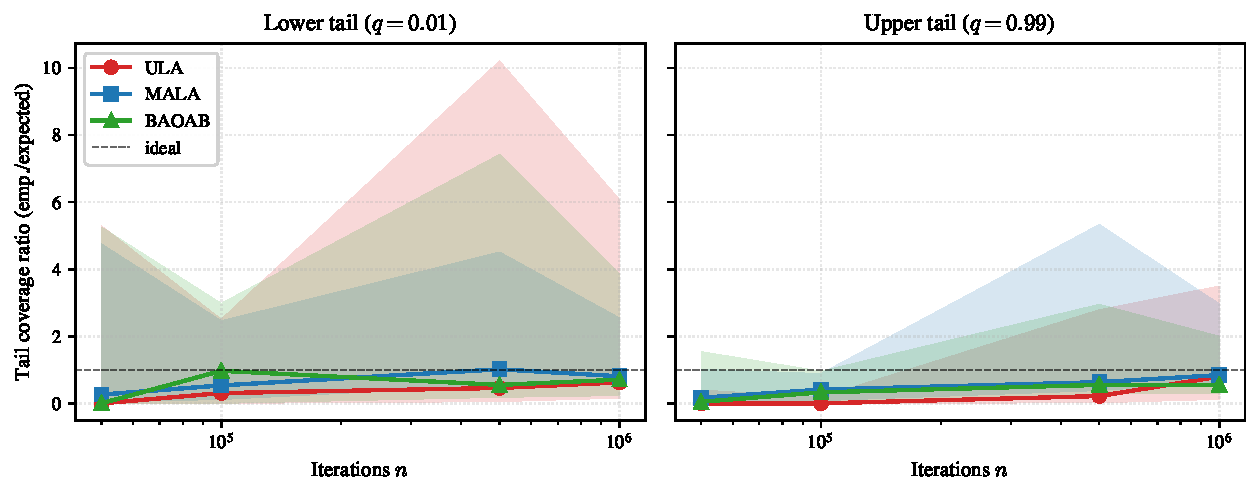
\includegraphics[width=\textwidth]{../../experiments/figures/original_thesis/cauchy_tail_coverage}
\caption{Αναλογίες κάλυψης ουράς Cauchy στα ποσοστημόρια $1\%$ και $99\%$,
διάμεση τιμή μεταξύ $10$ εκτελέσεων με ζώνη εκατοστημορίου $[5\%, 95\%]$. Η οριζόντια
γραμμή στο $1.0$ σηματοδοτεί ιδανική κάλυψη.}
\label{fig:tail-cauchy}
\end{figure}

Και οι τρεις αλγόριθμοι πλησιάζουν την ιδανική κάλυψη $1.0$ από κάτω καθώς η
αλυσίδα μεγαλώνει. Στις $N=10^6$ επαναλήψεις οι διάμεσες τιμές κάλυψης ουράς είναι: MALA
$0.81$ στο $q=0.01$ και $0.84$ στο $q=0.99$, BAOAB $0.71$ και $0.55$ αντίστοιχα, 
ULA $0.63$ και $0.80$. Ο MALA πλησιάζει περισσότερο την ιδανική κάλυψη, αλλά
οι ζώνες εκατοστημορίου $[5\%, 95\%]$ είναι πλατιές και για τους τρεις
αλγορίθμους --- ορισμένες εκτελέσεις δίνουν καλύψεις κοντά στο μηδέν, άλλοι πάνω
από τη μονάδα. Αυτή η μεταβλητότητα μεταξύ εκτελέσεων είναι εγγενής στην Cauchy:
οι εκτιμητές ακραίων ποσοστημορίων σε κατανομές βαριάς ουράς έχουν κατανομές
δειγματοληψίας βαριάς ουράς, και ακόμη και μια σωστά συμπεριφερόμενη αλυσίδα
παράγει άγρια διαφορετικές εκτιμήσεις κάλυψης ουράς μεταξύ διαφορετικών
εκτελέσεων.

Η οπτικοποίηση διασποράς εκτελέσεων στο Σχήμα~\ref{fig:seed-spread} το δείχνει
αυτό άμεσα: κάθε λεπτή γραμμή είναι η τροχιά KS μιας από τις δέκα εκτελέσεις ανά
αλγόριθμο για την Cauchy, ενώ η μέση τροχιά ανά αλγόριθμο αποδίδεται με έντονη γραμμή.
Η οικογένεια MALA έχει ένα σφιχτό κεντρικό σύμπλεγμα με λίγα ακραία σημεία.
Η οικογένεια BAOAB έχει ευρύτερη κεντρική διασπορά. Η οικογένεια ULA έχει τη
χαλαρότερη διασπορά από όλες.

\begin{figure}[ht]
\centering
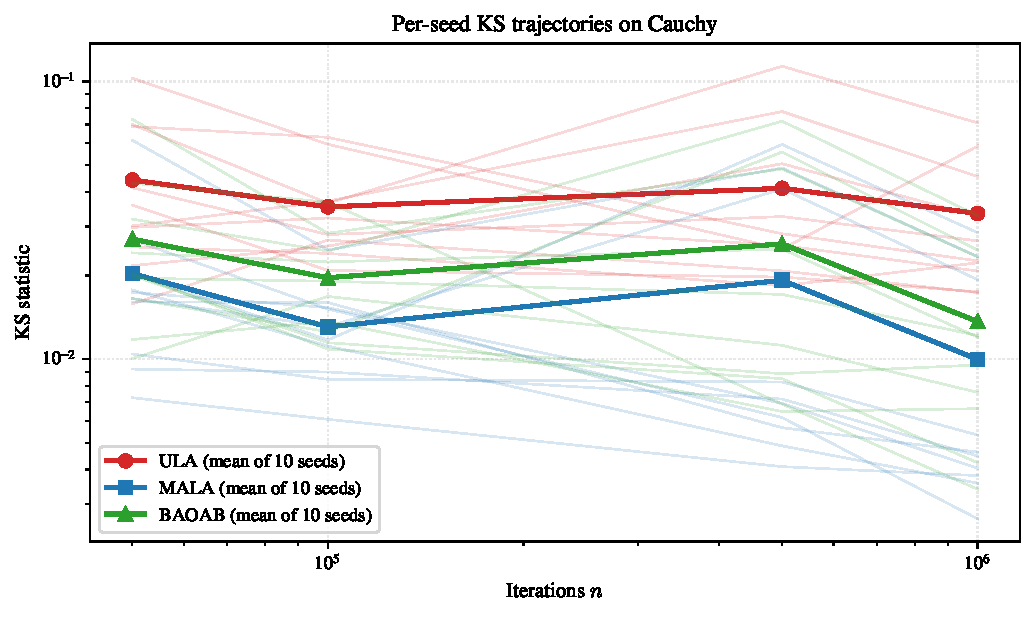
\includegraphics[width=0.75\textwidth]{../../experiments/figures/original_thesis/seed_spread_cauchy}
\caption{Τροχιές KS ανά εκτέλεση για την Cauchy κατανομή-στόχο. Οι αχνές γραμμές
αντιστοιχούν σε μεμονωμένες εκτελέσεις. Οι έντονες γραμμές είναι η μέση τροχιά
ανά αλγόριθμο.}
\label{fig:seed-spread}
\end{figure}

\subsection{Σύνοψη της Μελέτης Σύγκλισης}

Τρία συνοπτικά συμπεράσματα:

\begin{enumerate}
  \item Στα καθεστώτα ελαφριάς και μέτριας ουράς, ο MALA και ο BAOAB συγκλίνουν
        αμφότεροι κοντά στον γνωστό ρυθμό $1/\sqrt{N}$. Ο ULA κυριαρχείται από
        την μεροληψία διακριτοποίησης και συγκλίνει πολύ πιο αργά σε μια ελαφρώς
        λανθασμένη στάσιμη κατανομή.
  \item Για την Cauchy κατανομή-στόχο, ο MALA συνεχίζει να συγκλίνει κοντά στον
        ρυθμό $1/\sqrt{N}$. Ο BAOAB συγκλίνει περίπου με τον μισό αυτόν τον
        ρυθμό. Ο ULA μόλις κινείται. Από τους τρεις, ο MALA έχει τη χαμηλότερη
        απόλυτη KS στο $N=10^6$.
  \item Ωστόσο, το q-MAE της Cauchy στις $10^6$ επαναλήψεις ευνοεί τον BAOAB
        ($2.04$ έναντι $4.74$ του MALA), και η κάλυψη ουράς είναι παρόμοια μεταξύ
        των δύο. Η επιλογή βέλτιστου αλγορίθμου για την Cauchy εξαρτάται από το
        αν η εφαρμογή βαραίνει την προσαρμογή κορμού ή την ακρίβεια ουράς.
\end{enumerate}


\section{Επιφυλάξεις και Περιορισμοί}
\label{sec:caveats}

Κλείνουμε με κάποιες επιφυλάξεις που οριοθετούν τα συμπεράσματα αυτού του
κεφαλαίου.

\begin{enumerate}
 \item \emph{Είκοσι εκτελέσεις για τη μελέτη πλέγματος, δέκα για τη
        μελέτη σύγκλισης.} Ο αριθμός εκτελέσεων είναι αρκετός για να                                                          
        εντοπίσει μεγάλες διαφορές μεταξύ αλγορίθμων, αλλά όχι πολύ μικρές:
        διαφορές μικρότερες από $0.0005$ σε διάμεσο KS δεν είναι αξιόπιστες.
        Αρκετές συγκρίσεις BAOAB-έναντι-MALA στη Γκαουσιανή και τη
        Student-$t$ εμπίπτουν εντός αυτού του ορίου και θα πρέπει να
        θεωρούνται ισοπαλία.

  \item \emph{Η Cauchy δεν έχει πεπερασμένο μέσο ή διακύμανση.} Για τις
        εκτελέσεις Cauchy, οι μετρικές που βασίζονται σε μέσο και διακύμανση
        δεν έχουν νόημα και εμφανίζονται ως \texttt{NaN}. Η σύγκριση
        αλγορίθμων στην Cauchy γίνεται αποκλειστικά μέσω KS, διαμέσου και
        ποσοστημορίων.

  \item \emph{Το πλέγμα βήματος είναι διακριτό και εξαρτώμενο από την κατανομή.} Δοκιμάσαμε έναν
        συγκεκριμένο αριθμό τιμών $\eta$, οπότε το «βέλτιστο» που αναφέρουμε
        είναι το καλύτερο μέσα σε αυτό το πλέγμα, όχι το απόλυτο βέλτιστο.
        Για $d = 100$, μερικές από τις βέλτιστες τιμές βρίσκονται στο άκρο
        του πλέγματος --- κυρίως για BAOAB στη Γκαουσιανή και MALA στην
        Cauchy --- πράγμα που σημαίνει ότι μια ελαφρώς μεγαλύτερη ή
        μικρότερη τιμή $\eta$ θα μπορούσε να αποδώσει καλύτερα. Τα κύρια
        συμπεράσματα για τη συμπεριφορά των αλγορίθμων ως προς τη διάσταση
        δεν επηρεάζονται.

   \item \emph{Οι κατανομές-στόχοι είναι ισοτροπικές.} Και οι τρεις
        κατανομές-στόχοι αντιμετωπίζουν όλες τις διαστάσεις ισότιμα: δεν
        υπάρχουν διαστάσεις με διαφορετική κλίμακα ούτε συσχετίσεις μεταξύ
        τους. Στην πράξη, πολλά Bayesian προβλήματα δεν έχουν αυτή την
        ιδιότητα. Σε ανισοτροπικές κατανομές-στόχους η κατάταξη μεταξύ MALA
        και BAOAB μπορεί να αλλάξει, ειδικότερα το πλεονέκτημα ESS του BAOAB
        σε υψηλές διαστάσεις ενδέχεται να εξαφανιστεί χωρίς προρρύθμιση.

  \item \emph{Η μελέτη σύγκλισης είναι μόνο στο $d=1$.} Η μελέτη πλέγματος
        καλύπτει $d \in [1, 100]$ αλλά η μελέτη σύγκλισης που
        περιγράφεται στην Ενότητα~\ref{sec:convergence-study} διατηρεί $d=1$ για
        να απομονώσει τις επιδράσεις μήκους αλυσίδας από τις επιδράσεις
        διάστασης. Η παρατήρηση ότι και οι τρεις αλγόριθμοι καταρρέουν για την
        Cauchy μεταξύ $d=10$ και $d=100$ αποτελεί επομένως δήλωση σχετικά με
        ποιότητα αλυσίδας στις $5 \times 10^4$ επαναλήψεις. Μπορεί ή μπορεί να
        μην ισχύει εάν οι αλυσίδες τρέξουν πολύ περισσότερο σε υψηλό $d$.
 
\end{enumerate}

Παρά τους παραπάνω περιορισμούς, τα κύρια ευρήματα ισχύουν: ο ULA υποφέρει
από μόνιμη μεροληψία, ο MALA αποδίδει καλά σε όλες τις κατανομές, και ο BAOAB
κρατάει υψηλό ESS σε υψηλές διαστάσεις και καλύτερα ακραία ποσοστημόρια στις
βαριές ουρές.